\documentclass[../thesis.tex]{subfiles}
% !TeX spellcheck = fr_FR

\begin{document}
	
	\chapter{Détection des individus}
	\label{chap:deep-leaf}
    
    Après avoir séparé la végétation du reste de l'image, l'étape suivante vise à isoler des individus au sein de la végétation. Les algorithmes pouvant être utilisés pour cette opération ont été introduits dans la section \ref{sec:segmentation}. Toutefois, le choix de l'algorithme adéquat dépend du type d'entité recherchée. Il est en effet possible de s'intéresser à une composante connexe, une plante, une feuille, un super-pixel ou encore à un simple pixel. 
    
    Dans le cadre du challenge RoSE, la densité des plantes est importante. Il existe souvent un recouvrement entre les plantes (figure \ref{fig:07-beans-mustard-mix}). Si l'on définit l'entité comme étant une composante connexe, alors cette entité correspondra parfois à un amas de plantes (quand il y a recouvrement) et parfois à une plante isolée. Cela induira des erreurs d'étiquetage pour les amas de plantes, donc une classification grossière et l'impossibilité de détecter les adventices intra-rang, ce qui est l'objectif initial du challenge. A contrario, si nous définissons une segmentation au niveau du pixel, alors nous manquerons de propriétés pour une classification cultures/adventices performante.
    
    Les problématiques de segmentation, de caractérisation et de classification sont fortement liées. En réalité, la définition d'une méthode permettant d'obtenir un niveau de segmentation adéquat pour la classification culture/adventices constitue l'un des verrous scientifiques majeurs de cette thèse.
    
    \begin{figure}[H]
        \centering
        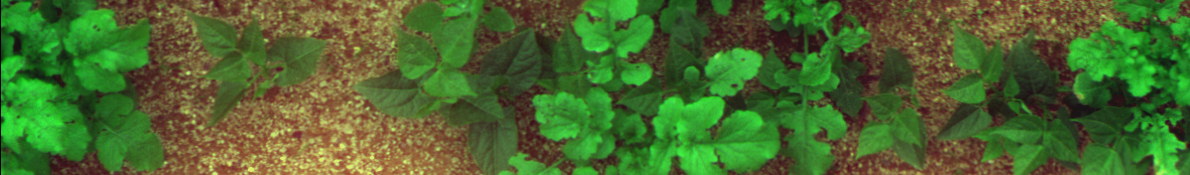
\includegraphics[width=\linewidth]{img/leaf-plus/beans-mustard-mix}
        \caption{Mélange de haricot (culture) et de moutarde (adventice) dans le challenge RoSE}
        \label{fig:07-beans-mustard-mix}
    \end{figure}
    
    
    Ainsi, dans notre contexte d'utilisation, en proxidétection, l'échelle de la composante connexe et celle du pixel sont à rejeter. L'échelle du superpixel pourrait être intéressante, en revanche, les algorithmes permettant une telle segmentation, sont longs et peu fiables, car fortement influencés par un paramètre essentiel, celui de la taille des superpixels. En effet, trop petits, les superpixels sont trop nombreux et ne contiennent pas suffisamment d'information discriminante. Trop grands, ils sont alors constitués de mélanges des classes culture et adventice.
    
    En agriculture de précision, pour la détection des adventices, l'entité de la plante est fréquemment utilisée. En effet, d'un point de vue agronomique, la plante est l'entité la plus fine utilisée pour caractériser, entre autres, l'état sanitaire et la pression des adventices.
    
    Les approches historiques de segmentation ne permettent pas de segmenter une entité plante de manière stable en conditions réelles car les images présentent de fortes variations. De plus, les tailles et formes des plantes varient fortement entre individus au sein d'une même espèce, ce qui rend tout processus d'optimisation préalable impossible sur des algorithmes tels que les superpixels. C'est pourquoi, aujourd'hui, l'essentiel de la communauté a recours à des algorithmes reposant sur de l'apprentissage profond.
    
    \newpage
    Les algorithmes d'apprentissage profond pris en considération en agriculture de précision utilisent des réseaux de neurones convolutifs (CNN) associés à une proposition des régions d'intérêts. Ces algorithmes de proposition de régions examinent une image d'entrée à travers un ensemble de convolutions qui maximisent l'identification de l'emplacement potentiel d'un objet. Cette méthode repose sur une régression de ``bounding box'', telle que proposée par \cite{girshick2014rich} (RCNN) ou \cite{app10020612} (YOLO).
    
    \begin{figure}[H]
        \centering
        {\scriptsize (source: \cite{app10020612})} \\
        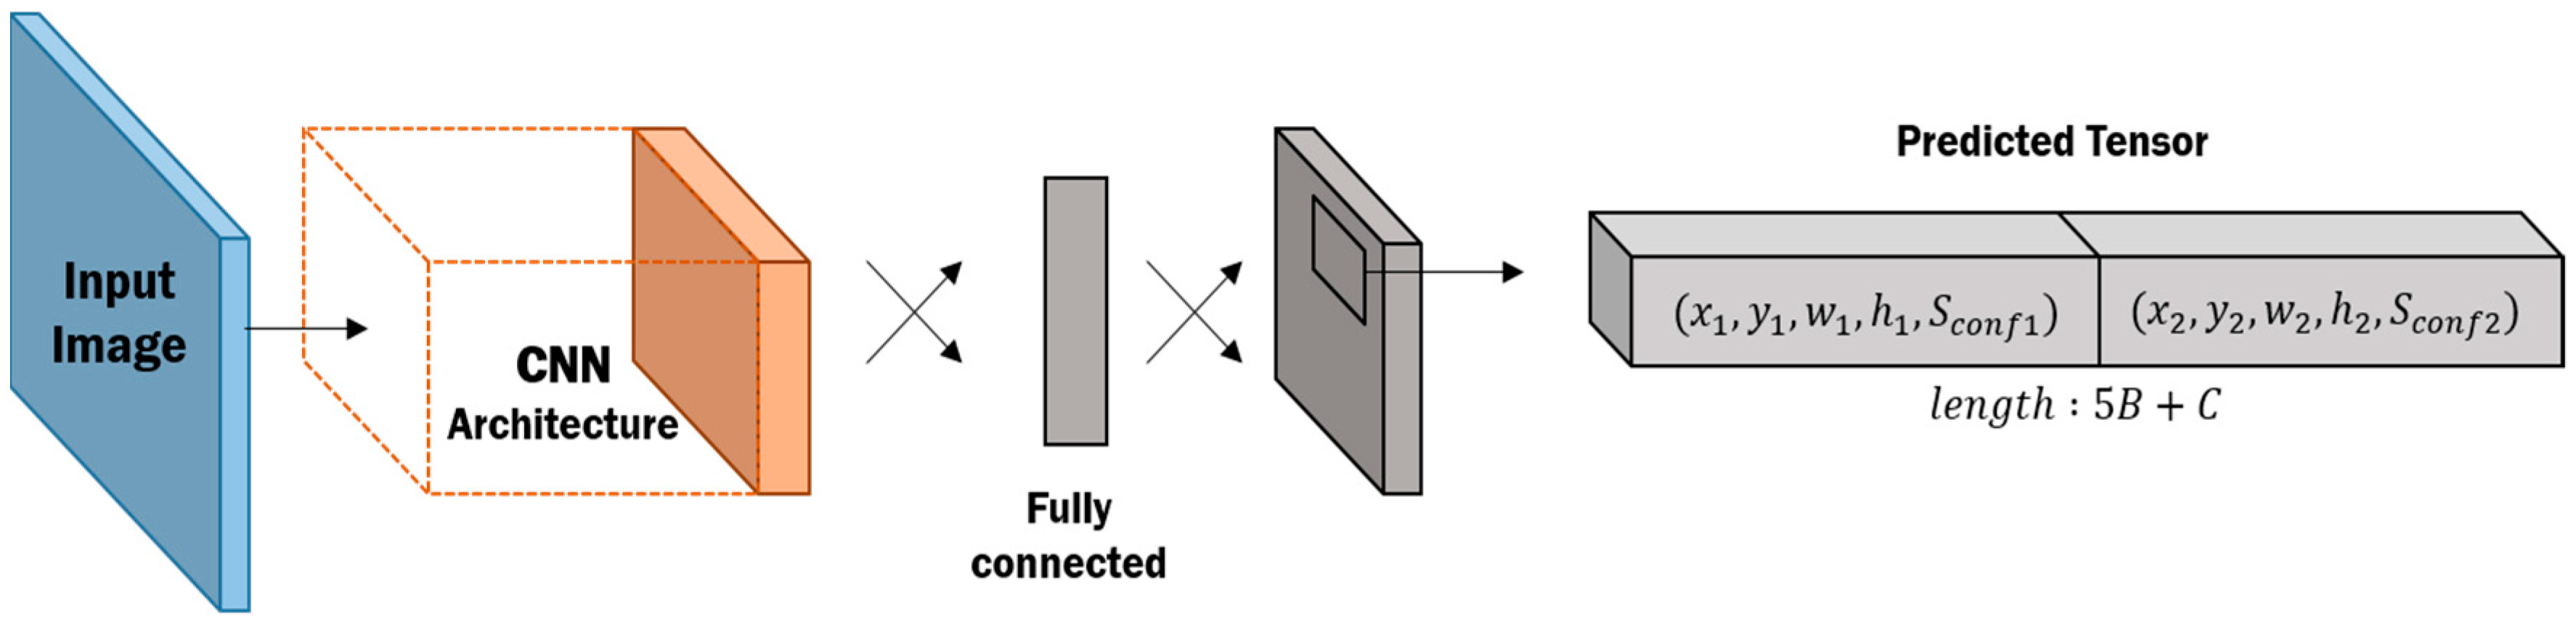
\includegraphics[width=0.7\linewidth]{img/biblio/segmentation-object}
        \caption{Structure d'un réseau ``You Only Look Once'' (YOLO)}
        \label{fig:07-03-segmentation-object}
    \end{figure}
    
    Les premiers travaux de \cite{girshick2014rich} utilisaient ensuite ces régions d'intérêt pour extraire les caractéristiques de sortie du réseau de neurones, afin de les introduire dans une machine à vecteurs de support (SVM) pour la classification finale. Au fil des évolutions, la classification SVM a été remplacée par un réseau de neurones dédié à l'identification de la classe de l'objet \cite{girshick2015fast}, permettant un apprentissage dit de ``bout en bout''. Cette régression des régions d'intérêt a toutefois deux inconvénients : (1) elle propose une grande quantité de faux positifs et (2) des sorties multiples, mais légèrement décalées, pour un même objet. Pour pallier ces problèmes, le ``score detection'' est utilisé pour supprimer la majorité des faux positifs, ainsi qu'un algorithme de suppression des non-maximum (NMS). Le NMS permet d'éviter la détection répétée de la même instance en combinant les régions (bounding box) qui se chevauchent en une seule boîte englobante pour chaque objet.
    
    Hélas, ce type d'approche montre ses limites en environnement dense, du fait de l'algorithme NMS. Ainsi, détecter des plantes par cette méthode ne permet pas un résultat optimal dans le cadre du challenge RoSE. En réalité, de par les nombreuses occultations et recouvrements inter-individus, l'échelle de la plante est discutable. De ce constat, il a été décidé de travailler sur une entité plus petite : la feuille. De plus, nous proposons ici, le développement d'un réseau de neurones ne s'appuyant pas sur l'algorithme NMS pour contourner ces limitations.
    
    En allant plus loin sur les réseaux de neurones définis pour les indices de végétation et la segmentation sol/végétation, il est possible de proposer un réseau de segmentation sémantique pour la segmentation des instances des feuilles. L'approche repose sur la détection des contours des feuilles \cite{morris2018pyramid}. Cette approche est peu utilisée mais elle peut être améliorée de différentes façons. La suite de ce chapitre porte sur les travaux qui ont été menés dans ce domaine pour développer une méthode de segmentation de feuille en couvert dense (chevauchement d'objets) et est l'objet d'une publication internationale dans la revue \textit{Computers and Electronics in Agriculture} (travail en cours de révision). % Ces travaux portent sur la détection de 4 classes, le contour des grandes feuilles, la séparation intérieure des grandes feuilles, les petites feuilles et l'intérieur des grandes feuilles.
	
	\newpage
    \null
    \vfill
	\section*{Pixelwise Instance Segmentation Of Leaves In Dense Foliage}
	
	\noindent
	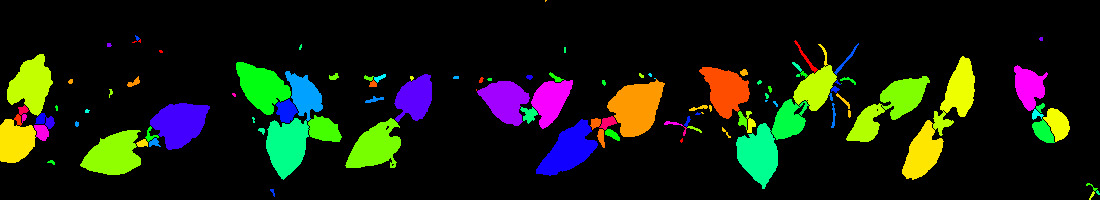
\includegraphics[width=\linewidth]{img/leaf/graphical-gca}
	
	\paragraph{Authors} Jehan-Antoine Vayssade, Gawain Jones, Christelle Gée and Jean-Noël Paoli
	
	\paragraph{Publication} Sent on 20/08/2021 -- Computer and Enlectronics in Agriculture -- under-review  %en cours de révision
		
	\paragraph{Abstract}
    Detecting and identifying plants using image analysis is a key step for many applications in precision agriculture (from phenotyping to site specific weed management). Instance segmentation is usually carried on to detect entire plants. However, the shape of the detected objects changes between individuals and growth stages. A relevant approach to reduce these variations is to narrow the detection on the leaf. Nevertheless, segmenting leaves is a difficult task, when images contain mixes of plant species, and when individuals overlap, particularly in an uncontrolled outdoor environment. To leverage this issue, this study based on recent Convolutional Neural Network mechanisms, proposes a pixelwise instance segmentation to detect leaves in dense foliage environment. It combines ``deep contour aware'' (to separate the inner of big leaves from its edges), ``Leaf Segmentation trough classification of edges'' (to separate instances with a specific inner edges) and ``Pyramid CNN for Dense Leaves'' (to consider edges at different scales). But the segmentation output is also refined using a Watershed and a method to compute optimized vegetation indices (DeepIndices). The method is compared to others running the leaf segmentation challenge (provided by the International Network on Plant Phenotyping) and applied on an external dataset of Komatsuna plants.  In addition, a new multispectral dataset of 300 images of bean plants is introduced (with dense foliage, individuals overlapping, mixes of species and natural lighting conditions). The ground truth (e.g. the leaves boundaries) is defined by labelled polygons and can be used to train and assess the performance of various algorithms dedicated to leaf detection or crop/weed classification. On the usual datasets, the performances of the proposed method are similar to those of the usual methods involved in the leaf segmentation challenges. On the new dataset, their results are strongly better than those of the usual RCNN method. Remaining errors are bad fusion between neighboring areas and over segmentation of multi-foliate leaves. Structural analysis methods could be studied in order to overcome these deficiencies.
    
    \paragraph{Keywords} precision agriculture ; remote sensing ; leaf segmentation ; dense foliage ; boundary detection ; semantic segmentation ; CNN ; multispectral
    \vfill
	
	\newpage
	\section{Introduction}
	
	In precision agriculture, one of the hardest tasks is the detection of crops and weeds by imagery. Imaging systems will play a significant role in the new generation of agriculture, from the genetic selection in phenotyping \cite{phenotyping} to site-specific weed management \cite{Louargant2017}. They are also used to record frequently and accurately the plant growth, crop yield, leaf area, etc \cite{Gee2021}. These data are then used to quantify and evaluate the quality of production.
    
    In proximal detection, this work is mainly done at the plant level and gives important agronomic information once reported at the plot level (number of weeds, crops and weeds locations,diseases, stress ...). The plant level is also needed for the new agricultural revolution, such as robotic weed management. Thus, studies try to detect crop and weeds plants by using a wide variety of techniques, which have been reviewed by \cite{WANG2019226}. The instance segmentation is a key-step used before the task of classifying plants as crop and weeds. In CNN field, it is mostly based on a major class approaches \cite{Hafiz_2020}, such as Mask-RCNN. However, detecting the entire plants has 3 main limitations (i) when plants are too numerous, it is hard to distinguish individuals when they overlap, one of them is undetected or both are merged which is due to the underlying non-max suppression algorithm \cite{BONNEAU2020105150}, (ii) small and thin elements are undetected and (iii) the number of variations for a plant is infinite: the number of leaves, their orientations, their sizes and other differences that radically change between individuals and growth stages, implies a large amount of data for the training process. These limitations logically impact the detection rate and may cause a significant quantity of miss-detection. To solve this problem, one approach that should be relevant is to base the detection not on the whole plant, but on the leaf. For this purpose, a pixel-wise instance segmentation is proposed. The idea is to separate the instances by detecting the edges of the leaves whose projected shadow gives an interesting gradient break, particularly in an uncontrolled outdoor environment.
    
    \subsection{Related Works}
    
    Some recent works on leaf segmentation were found in controlled illumination environments with limited occlusion between individuals. Especially on an open dataset of Arabidopsis Thaliana \cite{scharr2016leaf}. Other studies related to biomedical imagery and nuclei segmentation were also found with pixel-wise instance segmentation. These studies show the important of defining one or more edges classes and a relevant loss function. These two factors are both related to the weight given to each sample of the training dataset in the estimated error for the optimization algorithm. But the way of how parts of the network are dedicated to the edge classification and thus on how the network focuses on instance separation. Edge detection therefore plays a significant role in pixelwise instance segmentation task.
    
    \newpage
    The first studies were dedicated to the definition of specific class of edges to separate instances. Thus \cite{chen2016dcan} proposed a novel approach named ``Deep Contour-Aware'' based on the semantic segmentation of two classes, one class is dedicated to the inside of glands, while the second is for the segmentation of glands edges. A bit later, \cite{morris2018pyramid} was the first to define a pixelwise instance segmentation for dense leaf detection. They proposed the ``Pyramid CNN for Dense Leaves'' architecture which is similar to U-Net (the most common CNN used for biomedical images segmentation). The network is dedicated to the detection of leaf boundaries. To facilitate the learning of edges at different scales, an auxiliary loss function is placed at each sub-scale of the pyramid. Finally, the instances are retrieved by using a superpixel algorithm.
    
    \cite{Cui_2019} enhance the ``Deep Contour-Aware'' model proposed in 2016 by using a real U-Net architecture and data augmentation. Concerning edge classes based instances segmentation, \cite{bell2019leaf} study shows the importance of separating edges into two classes. As the outer edges are dominant in the samples, the corresponding error on contiguous edges are less important. Thus, the edges of leaves are separated into two classes, one for the outer edges and one for inner edges (when leaves are touching or overlapping). The multi-scale loss function is still used and proposed by \cite{xie2020instanceaware} for nucleus instance segmentation. They show that multi-scale loss helps to regularize the network and narrow down the perceptual distances and enlarge the semantic dissimilarity between individuals. In addition, a count ranking loss is used on the last feature layer of a fully-connected layer. This count ranking loss enforces the network to focus on the learning of samples containing crowded nuclei. This technique results in an implicitly regularized trained network, to be aware of individuals quantity.
    
    \subsection{Objectives}
    
    %% All these studies show a close relationship between the loss function and the defined semantic classes, they have shown that pixelwise instance segmentation technique is viable but still limited. Based on these related works, this paper proposes to merge most recent advances in the field of pixelwise instance segmentation. The proposed method combines ``deep contour aware'' (to separate the inner of big leaves from its edges), ``Leaf Segmentation trough classification of edges'' (to separate instances with a specific inner edges) and ``Pyramid CNN for Dense Leaves'' (to consider edges at different scales). A new loss function is also introduced to limit under and over-segmentation. The output is refined using a specific vegetation index based on previous work \cite{Vayssade2021}. This method is applied to dense leaf segmentation in a new multispectral image dataset presented in the next section. The method is also evaluated on two common online leaf RGB image databases \cite{scharr2016leaf}. The proposed method is much more robust compared to previous pixel-wise instance segmentation methods and solves the issue of methods based on bounding-box regression : all small and thin elements are detected.
    
    %% Highlights : 
    %% Pixelwise Instance segmentation of leaves is performed on mixes of plant species
    %% A new shape-based loss function is proposed and applied to each connected component
    %% The segmentation output is refined using a Watershed and a DeepIndices approach
    %% A benchmark of the method is performed on “leaf segmentation challenges”
    %% A new multi-spectral dataset of 300 images acquired in natural light is shared
    
    %% Au final, petite tentative de mixer les highlights et les objectifs. En parallèle je vous propose de changer un peu la hiérarchie des titres du 2 et du 3. L'idée c'est que chaque highlight corresponde à un niveau 2 et pas à un niveau 3.  Et ajout d'une petite phrase concernant la loss function dans l'intro du chapitre 3. 
    
    All these studies show  that pixelwise instance segmentation technique is viable but still limited. They also underline the importance of choosing a loss function adapted to the defined semantic classes. Based on these related works, this paper proposes to merge most recent advances in the field of pixelwise instance segmentation. 
    
    First, the proposed method combines ``deep contour aware'' (to separate the inner of big leaves from its edges), ``Leaf Segmentation trough classification of edges'' (to separate instances with a specific inner edges) and ``Pyramid CNN for Dense Leaves'' (to consider edges at different scales). Second, a new loss function is also introduced to limit under and over-segmentation. Third output is refined using a specific vegetation index based on previous work \cite{Vayssade2021} and a watershed algorithm. 
    
    This method is applied to dense leaf segmentation, on images containing mixes of plant species and acquired in natural light. A specific multispectral dataset has been acquired, it is presented in the next section \ref{sec:Airphen-dataset} and released publicly. The method is also evaluated on two common online leaf RGB image databases \cite{scharr2016leaf}, presented in section \ref{sec:online-dataset}. 
    
    The proposed method is much more robust compared to previous pixel-wise instance segmentation methods and solves the issue of methods based on bounding-box regression : all small and thin elements are detected.
    
    \newpage
    \section{Material and data}
    
    % 2.1. Specific multispectral dataset
    % 2.1.1. Experimental plot
    % 2.1.2. multispectral camera
    % 2.1.3. Image acquisition and annotation
    % 2.2. Online image databases
    % 2.2.1.  Additional data from the Computer Vision Problems... (CVPPP)
    % 2.2.2.  Additional data from Komatsuna dataset
    
    \subsection{Specific multispectral dataset}
    \label{sec:Airphen-dataset}
    \subsubsection{Experimental plot}
    
    The data were acquired at the site of INRAE (Figure \ref{fig:07-parcelle-xp}) in Montoldre (Allier, France, at 46°20'30.3”N 3°26'03.6”E) within the framework of the “RoSE challenge” founded by the French National Research Agency (ANR) in 2019. The aim of the Challenge is to objectively compare the solutions proposed by participants for intra-row weed control (\cite{ChallengeRoSE}). Within this context, the challenge provides to contestants an evaluation plan and a set of experimental plots of bean and maize plants. In addition various natural weeds (yarrows, amaranth, geranium, plantago, etc) and sown ones (mustards, goosefoots, mayweed and ryegrass) are managed to compare performances.
    
    \begin{figure}[H]
        \centering
        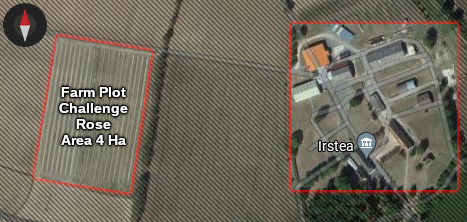
\includegraphics[width=0.5\linewidth]{img/leaf/parcelle-xp}
        \caption{Aerial view of the experimentation plot located in Montoldre (now INRAE)}
        \label{fig:07-parcelle-xp}
    \end{figure}
    
    \subsubsection{multispectral camera}
    
    The images were acquired with the Airphen (Hyphen, Avignon, France) six-band multispectral camera (visible on the upper-left of the Figure \ref{fig:07-trecktor}). This is a scientific camera developed by agronomists for agricultural applications. The camera embeds six sensors using six bandpass (450/570/675/710/730/850 nm) filters with a 10 nm FWHM each. The focal length of each lens is 8 mm. The raw resolutions for each spectral band are $1280 \times 960$ px with 12 bit precision. Due to the conception of the camera, spectral images are not aligned. Based on previous work \cite{vayssade:hal-02499730}, a method for registration has been developed with a registration accuracy down to sub-pixel. After the registration, all spectral images are cropped to 1200*800 px and concatenated to channel-wise where each dimension refers to a spectral band.
    
    %\begin{figure}[H]
    %	\centering
    %	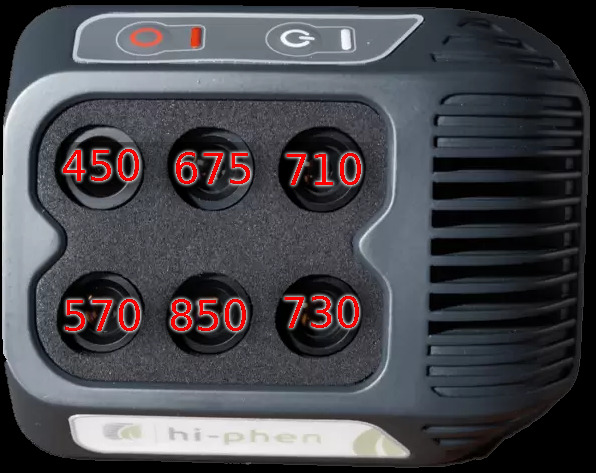
\includegraphics[height=7em]{img/leaf/camera-airphen}
    %	\caption{The Airphen six spectral band camera}
    %	\label{fig:07-camera-Airphen}
    %\end{figure}
    
    
    \subsubsection{Image acquisition and annotation}
    
    From the presented experimental plots, a set of images were acquired. The camera is attached in front of an hybrid autonomous tractor called “TREKTOR” launched by SITIA Company (Bouguenais, France) in 2019. The camera is setup to have a top-down view of crop rows, thus it is mounted on a pole in front of the platform allowing to remove visible part of the robot and at 1.8 m from the ground. The Figure \ref{fig:07-trecktor} below shows the arrangement of the elements. Crops and weeds were between phenological state 3 and 4 which means they have between 2 and 6 leaves. The ground truth is defined on images by experts with polygons around each leaf boundary. In addition, polygons contain a label for their classification between crop and weed (not used in this study). The annotation was defined using the VIA annotation software \cite{dutta2019vgg} and a total of 300 images of bean were annotated, 170 from acquisition made in June and 130 in October. These dataset is freely available at \url{https://doi.org/10.15454/JMKP9S}.
    
    \begin{figure}[H]
        \centering
        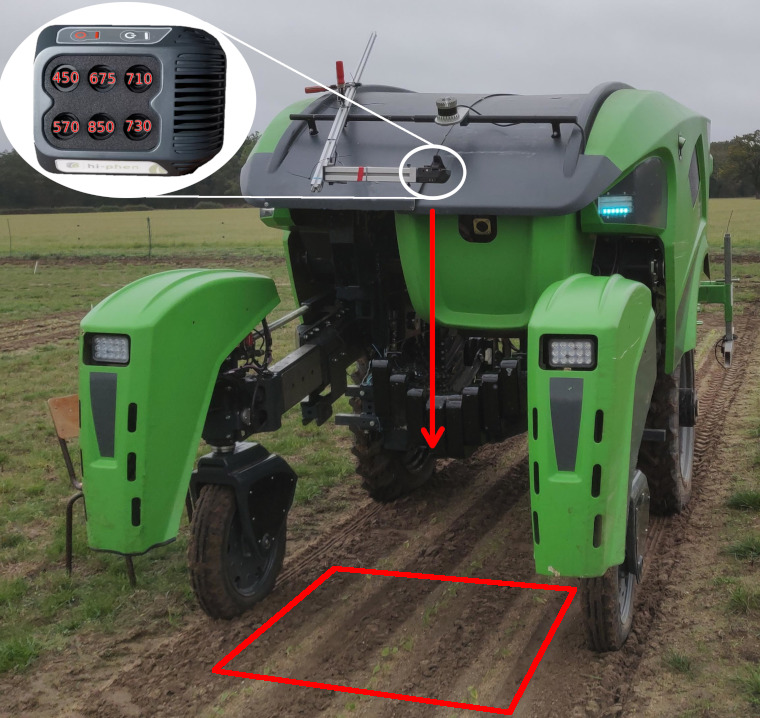
\includegraphics[width=0.5\linewidth]{img/leaf/trektor}
        \caption{The experimental set-up : the multispectral camera and the robotic plateform}
        \label{fig:07-trecktor}
    \end{figure}
    
    \subsection{Online image databases}
    \label{sec:online-dataset}
    
    \subsubsection{Additional data from the Computer Vision Problems in Plant Phenotyping dataset (CVPPP)}
    \label{sec:cvppp-dataset}
    
    To compare the method proposed in this study with others, an additional dataset was used. This dataset is proposed for the Leaf Segmentation Challenge (LSC \cite{scharr2017computer})  provided by the International Network on Plant Phenotyping (INPP), a very popular challenge for data scientists. It is composed of RGB images of Arabidopsis Thaliana (783 images) and Rosette (27 images) plants segmented into several leaves. The authors state that the images were collected from multiple locations in a growth chamber experiment and divided into four groups, named A1 through A4. In addition, the dataset is composed of various image sizes (respectively $530 \times 530, 565 \times 565, 2048 \times 2048, 441 \times 441$ for each sub-dataset), which have been resize to $512 \times 512 \times 3$. % \footnote{online CVPPP dataset at \url{https://competitions.codalab.org/competitions/18405}}
    
    \begin{figure}[H]
        \centering
        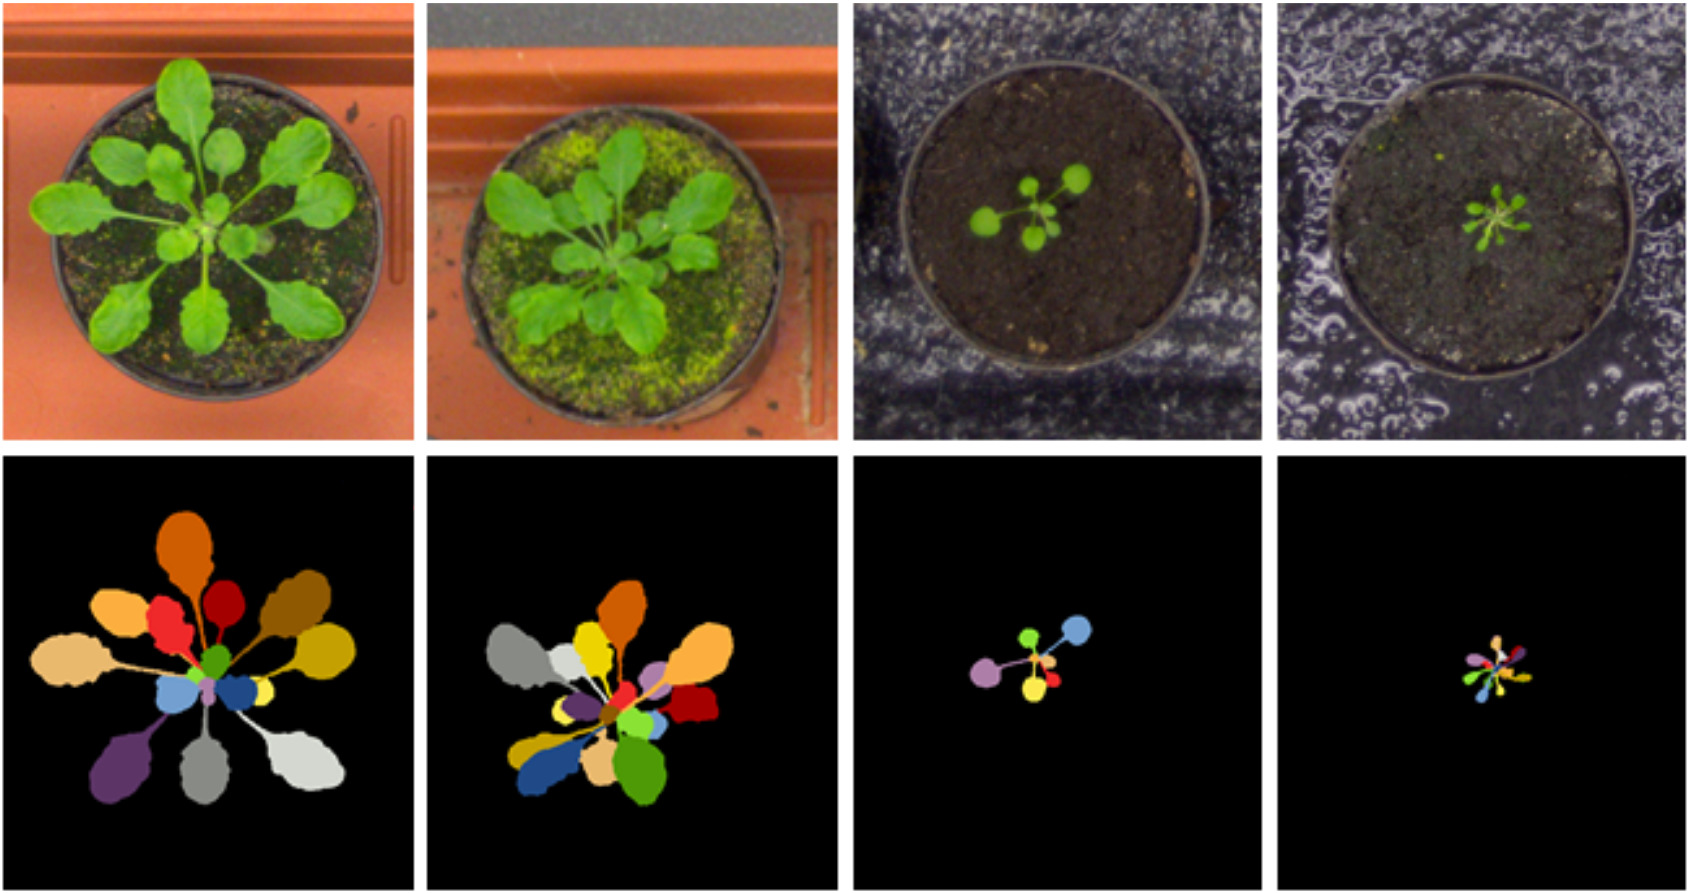
\includegraphics[width=0.7\linewidth]{img/leaf/dataset-cvppp}
        \caption{Example of images from the CVPPP dataset (top) and their corresponding ground truth (bottom)}
        \label{fig:07-dataset-cvppp}
    \end{figure}
    
    
    \subsubsection{Additional data from Komatsuna dataset}
    \label{sec:komatsuna-dataset}
    
    Similar to the LSC dataset, Komatsuna dataset consists in RGB images of plants taken in a top view. This dataset contains a large number of plant growth stages, it was designed to solve the problem of 3D phenotyping \cite{Uchiyama_2017_ICCV_Workshops}. It is used here primarily as a test set due to its similarity to the CVPPP dataset (training set), as shown in Figure \ref{fig:07-dataset-komatsuna}. This dataset includes 900 images of size $480 \times 480 \times 3$. % \footnote{online Komatsuna dataset at \url{https://limu.ait.kyushu-u.ac.jp/~agri/komatsuna/}}
    
    \begin{figure}[H]
        \centering
        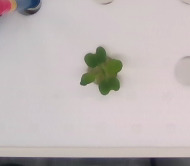
\includegraphics[width=0.2\linewidth]{img/leaf/dataset-Komatsuna-rgb-1}
        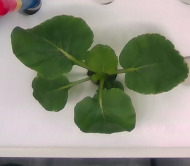
\includegraphics[width=0.2\linewidth]{img/leaf/dataset-Komatsuna-rgb-2}
        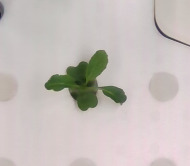
\includegraphics[width=0.2\linewidth]{img/leaf/dataset-Komatsuna-rgb-3}
        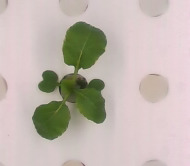
\includegraphics[width=0.2\linewidth]{img/leaf/dataset-Komatsuna-rgb-4} \\
        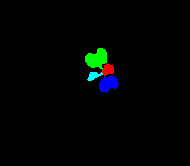
\includegraphics[width=0.2\linewidth]{img/leaf/dataset-Komatsuna-label-1}
        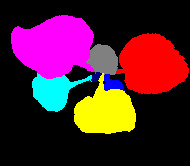
\includegraphics[width=0.2\linewidth]{img/leaf/dataset-Komatsuna-label-2}
        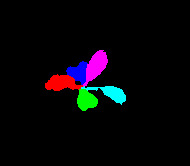
\includegraphics[width=0.2\linewidth]{img/leaf/dataset-Komatsuna-label-3}
        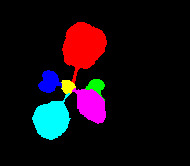
\includegraphics[width=0.2\linewidth]{img/leaf/dataset-Komatsuna-label-4} \\
        \caption{Example of RGB images from the  Komatsuna dataset (top) and their corresponding ground truth (bottom)}
        \label{fig:07-dataset-komatsuna}
    \end{figure}
    
    
    \section{Methodology}
    
    We consider the leaf segmentation as a binary segmentation problem of boundaries as proposed by \cite{morris2018pyramid}. The main idea is to detect the sharp edges of leaves or to follow the projected shadow of a leaf on the one below it. This methodology section is split into three sub-tasks (\ref{sec:proposed-cnn}) the proposed CNN architecture to detect and separate leaves, (\ref{sec:loss-function}) the specific loss function defined to limit under and over-segmentation, and (\ref{sec:watershed-refinement}) a simple watershed algorithm which takes the CNN output and a vegetation mask to refine the segmentation. %, also proposed by \cite{sapoukhina2019data}.
    
    % 3.1.  Proposed CNN architecture
    % 3.1.1.  Upstream of the network
    % 3.1.2.  Core network model
    % 3.1.3.  Downstream of the network
    % 3.2. Loss function
    % 3.3.  Refinement with vegetation mask and watershed
    
    \subsection{Proposed CNN architecture}
    \label{sec:proposed-cnn}
    
    Unlike recent CNN architectures, the proposed approach is slightly more decomposed like standard biomedical and agricultural computer vision pipelines \cite{pmid29048559, 8206403}. Thus, the architecture (Figure \ref{fig:07-diagram1}) is composed of three \textbf{upstream modules} (IIT, IBF, UFA) that improves the input data and eliminates unnecessary information. This step composed of 3 \textbf{upstream} modules, was proposed in a previous work to construct a vegetation index (\cite{Vayssade2021}). It is used to identify relevant spectral features on the input data to exploit the inter-channel relationships. After this stage, a \textbf{core network} is used to consider spatial information at different scales on the image, the core network returns four down-scaled feature maps. Finally, at the end of the network, three \textbf{downstream modules} (CoordConv, UFA, Classification) are proposed to fuse spectral and spatial information. Sigmoid activation function is used at the end of all convolution layers to learn more complex structures and allows non-linearity of the reconstructed function.
    
    \begin{figure}[H]
        \centering
        %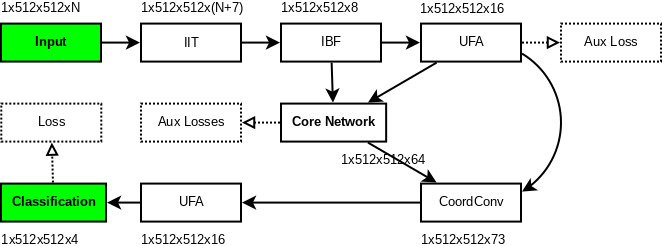
\includegraphics[width=\linewidth]{img/leaf/Diagram1}
        \tikzset{
	ppblock/.style={
		rectangle,
		minimum size=6mm,
		very thick,
		draw=black!50,
		text centered,
		font=\ttfamily,
		minimum width=8em,
		minimum height=6mm,
		top color=white,
	},
	%
	figure/.style={
		rectangle,
		rectangle split,
		rectangle split parts=2,
		very thick,
		draw=black!50,
		text centered,
		append after command={
			\pgfextra
			\fill[top color=#1, bottom color=#1]
			(\tikzlastnode.one west) 
			[rounded corners] |- (\tikzlastnode.north) -| (\tikzlastnode.one east) 
			[sharp corners]   |- (\tikzlastnode.one split) -| cycle;
			\fill[top color=white, bottom color=#1]
			(\tikzlastnode.two west) 
			[rounded corners] |- (\tikzlastnode.south) -| (\tikzlastnode.two east)  
			[sharp corners]   |- (\tikzlastnode.one split) -| cycle;
			\endpgfextra
		},
	},
    splitted/.style={
        rectangle,
        rectangle split,
        rectangle split horizontal,
        rectangle split parts=2,
        very thick,
        draw=black!50,
        text centered,
        append after command={
            \pgfextra
            \fill[top color=white, bottom color=#1]
            (\tikzlastnode.south)
            [rounded corners] -| (\tikzlastnode.west) |- (\tikzlastnode.one north)
            [sharp corners]   -| (\tikzlastnode.one split) |- cycle;
            \fill[top color=white, bottom color=#1]
            (\tikzlastnode.two south)
            [rounded corners] -| (\tikzlastnode.east) |- (\tikzlastnode.north)
            [sharp corners]   -| (\tikzlastnode.one split) |- cycle;
            \endpgfextra
        },
    },
	%
	static/.style={ppblock, bottom color={black!20}},
	nonterminal/.style={ppblock, bottom color={blue!30}},
	terminal/.style={ppblock, bottom color={green!20}},
	algorithm/.style={ppblock, bottom color={yellow!50}},
	error/.style={ppblock, bottom color={red!20}},
	type/.style={ppblock, bottom color={red!20}},
	loss/.style={ppblock, dashed, bottom color={black!20}, font=\itshape},
	%
	tiny/.style={
		rounded rectangle,
		very thick,
		draw=black!50,
		top color=white,
		bottom color=red!20,
        text centered,
		font=\ttfamily,
	},
    operator/.style = {
        circle,
        scale=0.6,
        draw=black!50,
        top color=white,
        bottom color=red!20,
        font=\boldmath,
    },
	%
	skip loop/.style={to path={-- ++(0,#1) -| (\tikztotarget)}}
}

\begin{tikzpicture}[
		>=stealth',thick,
		tip/.style={->,shorten >=0.007pt},
		every node/.style={scale=0.7},
		]
		\matrix[column sep=4mm, row sep=4mm, align=center] {
			% First row:
			\node (raw)    [terminal]      {Input \\ 1x512x512xN};         &
			\node (iit)    [nonterminal]   {IIT \\ 1x512x512x(N+7)};           &
			\node (ibf)    [nonterminal]   {IBF \\ 1x512x512x8};           &
			\node (ufa1)   [nonterminal]   {UFA \\ 1x512x512x16};           \\
			
			
			
			\node (loss3)   [loss]          {Loss};         &
			\node (loss2)   [loss]          {Aux Loss};     &
			\node (core)    [nonterminal]   {Core Network \\ 1x512x512x64}; \\
			
			
			\node (thr)    [terminal]      {Classification \\ 1x512x512x4};         &
			\node (ufa2)   [nonterminal]   {UFA \\ 1x512x512x16};                   &
			\node (coord)  [nonterminal]   {CoordConv \\ 1x512x512x73}; & 
			\node (loss1)  [loss]          {Aux Loss};      \\
		};
		
		\begin{scope}[->,rounded corners=2mm]
		\draw[->]     (raw) -- (iit);
		\draw[->]     (iit) -- (ibf);
		\draw[->]     (ibf) -- (ufa1);
		\draw[->]     (ufa1.south) to [in=45,out=-90] (coord.north east);
		
		\draw[->, dotted]     (ufa1) -- (loss1);
		\draw[->, dotted]     (ufa2) -- (loss2);
		\draw[->, dotted]     (thr) -- (loss3);
		
		\draw[->]     (ufa1.south west) -- (core.north east);
		\draw[->]     (core) -- (coord);
		\draw[->]     (coord) -- (ufa2);
		\draw[->]     (ufa2) -- (thr);
		\draw[->]     (ibf)  -- (core);
		\end{scope}
		
		\end{tikzpicture}
		\\
        \caption{Diagram of the CNN network architecture and losses (dotted). Multiple arrow show concatenation as input layer.}
        \label{fig:07-diagram1}
    \end{figure}
    
    The network takes an input image of size $512 \times 512 \times 6$, thus the learning and computation are done by a sliding window within the registered images of the Airphen camera of size  $1200 \times 800 \times 6$. The output layer is defined as a semantic segmentation of four classes. One class is dedicated to the inner of individuals, while three classes are dedicated to the detection of edges to keep aware of leaves instance. As mentioned by \cite{bell2019leaf}, one class is dedicated to outer of leaf (touching soil texture), while the second is dedicated to inner edges (touching/overlapping another leaf). Within our dataset, a third class appears with thin leaves which can be considered as a kind of edge. The ground truth is a set of polygons, drawn with the respect of these classes. Edge classes were empirically drawn with three pixel thickness. The following figure shows the input ground truth.
    
    \begin{figure}[H]
        \centering
        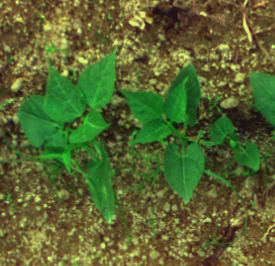
\includegraphics[width=0.25\linewidth]{img/leaf/dataset-color} \hspace{1em}
        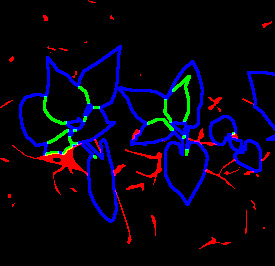
\includegraphics[width=0.25\linewidth]{img/leaf/dataset-edges} \hspace{1em}
        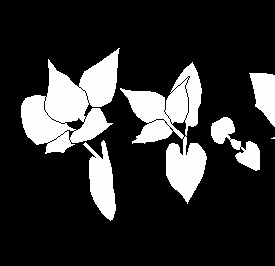
\includegraphics[width=0.25\linewidth]{img/leaf/dataset-body}
        \caption{Example of input data: from left to right, the first three bands (RGB) of the Airphen multispectral camera, three edge classes and the inner of individual class}
        \label{fig:07-dataset-body}
    \end{figure}
    
    \newpage
    \subsubsection{Upstream of the network}
    It is composed of three \textbf{upstream} modules: Initial Image Transforms (IIT), Input Band Filter (IBF) and Universal  Function  Approximator  (UFA).
    \paragraph{Initial Image Transforms (IIT)} In order to enrich the pool of information, spectral band transformations are added to take into account specific spatial gradients in the image and spectral mixing. Seven important transformations are considered. The standard deviation between spectral bands, noted $\rho_{std}$ can help to detect the spectral mixture. For example, between two different surfaces like ground and leaf (which have opposite spectral radiance), the spectral mixing makes a pixel with linear combination, thus the standard deviation tends to zero \cite{Louargant2017}. Three Gaussian derivatives on different orientations are computed. Gxx, Gxy and Gyy filters on $\rho_{std}$  give an important spatial information about the breaks of gradient, and therefore about the outer limits of surfaces. The Laplacian, the minimum and maximum eigenvalues (of the Hessian matrix) also called ridge of the $\rho_{std}$ seems to easily detect fine elements \cite{LinVessel}, such as monocotyledons for vegetation images. All these transformations are concatenated to the channel-wise normalized spectral band input and build the final input image. In the end we have six spectral images plus seven transformations for a final image composed of 13 channels.
    
    \paragraph{Input Band Filter (IBF)} To remove unneeded parts of the signal, low-pass, high-pass and band-pass filters are added. To apply the low-pass filter we use the equation $z = max(x-a,0)/(1-a)$ and thus it allows to suppress low values. For the high-pass filter we apply the equation $w = max(b-x,0)/b$ to suppress the high values. The band-pass filter is the product of low-pass and high-pass filters defined by $y = z*w$. The output layer is the concatenation in the channel-wise of the input images, the low-pass, the high-pass and the band-pass filter which produce 4*13 = 52 channels. Finally, to reduce the output data for the rest of the network, a bottleneck is inserted using a $3 \times 3$ convolution layer, and it generates a new tensor with 16 channels.
    
    \paragraph{Universal Function Approximator (UFA)} To separate efficiently leaves from the background and to learn spectral features, a Universal Function Approximator is defined on the upstream of the network (Figure \ref{fig:07-ufa}). The UFA is based on Taylor expansion theorem, an approach to learn this form of development in deep-learning is called DenseNet and then corresponds to the sum of the concatenation of the signal with these spatio-spectral derivatives. This was successfully used for vegetation segmentation \cite{Vayssade2021}. Three parameters, such as the $depth$ (number of convolutions), the $width$ (number of filters denoted $W$) and $k$ (kernel size) configure the network and were empirically fixed to $depth=3$, $width=16$ and $k=1$. An auxiliary output is used here to maximize the class similarity on the upstream of the network and to extract pure spectral information.
    
    \begin{figure}[H]
        \centering
        %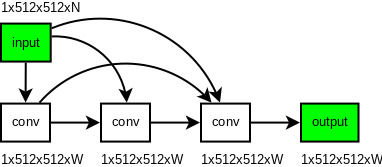
\includegraphics[width=0.6\linewidth]{img/leaf/Diagram3} \\
        \tikzset{
	ppblock/.style={
		rectangle,
		minimum size=6mm,
		very thick,
		draw=black!50,
		text centered,
		font=\ttfamily,
		minimum width=8em,
		minimum height=6mm,
		top color=white,
	},
	%
	figure/.style={
		rectangle,
		rectangle split,
		rectangle split parts=2,
		very thick,
		draw=black!50,
		text centered,
		append after command={
			\pgfextra
			\fill[top color=#1, bottom color=#1]
			(\tikzlastnode.one west) 
			[rounded corners] |- (\tikzlastnode.north) -| (\tikzlastnode.one east) 
			[sharp corners]   |- (\tikzlastnode.one split) -| cycle;
			\fill[top color=white, bottom color=#1]
			(\tikzlastnode.two west) 
			[rounded corners] |- (\tikzlastnode.south) -| (\tikzlastnode.two east)  
			[sharp corners]   |- (\tikzlastnode.one split) -| cycle;
			\endpgfextra
		},
	},
    splitted/.style={
        rectangle,
        rectangle split,
        rectangle split horizontal,
        rectangle split parts=2,
        very thick,
        draw=black!50,
        text centered,
        append after command={
            \pgfextra
            \fill[top color=white, bottom color=#1]
            (\tikzlastnode.south)
            [rounded corners] -| (\tikzlastnode.west) |- (\tikzlastnode.one north)
            [sharp corners]   -| (\tikzlastnode.one split) |- cycle;
            \fill[top color=white, bottom color=#1]
            (\tikzlastnode.two south)
            [rounded corners] -| (\tikzlastnode.east) |- (\tikzlastnode.north)
            [sharp corners]   -| (\tikzlastnode.one split) |- cycle;
            \endpgfextra
        },
    },
	%
	static/.style={ppblock, bottom color={black!20}},
	nonterminal/.style={ppblock, bottom color={blue!30}},
	terminal/.style={ppblock, bottom color={green!20}},
	algorithm/.style={ppblock, bottom color={yellow!50}},
	error/.style={ppblock, bottom color={red!20}},
	type/.style={ppblock, bottom color={red!20}},
	loss/.style={ppblock, dashed, bottom color={black!20}, font=\itshape},
	%
	tiny/.style={
		rounded rectangle,
		very thick,
		draw=black!50,
		top color=white,
		bottom color=red!20,
        text centered,
		font=\ttfamily,
	},
    operator/.style = {
        circle,
        scale=0.6,
        draw=black!50,
        top color=white,
        bottom color=red!20,
        font=\boldmath,
    },
	%
	skip loop/.style={to path={-- ++(0,#1) -| (\tikztotarget)}}
}

\vspace{-1em}
\begin{tikzpicture}[
	>=stealth',thick,
	tip/.style={->,shorten >=0.007pt},
	every node/.style={scale=0.7},
	]
	
	\matrix[column sep=4mm, row sep=4mm, align=center] {
		% First row:
		\node (raw)    [terminal]      {Input \\ 1x512x512xN};        &
		\node (conv1)  [nonterminal]   {Conv \\ 1x512x512xW};         &
		\node (conv2)  [nonterminal]   {Conv \\ 1x512x512xW};         &
		\node (conv3)  [nonterminal]   {Conv \\ 1x512x512xW};         &
		\node (out)    [terminal]      {Output \\ 1x512x512xW};       &
		\\
	};
	
	\begin{scope}[->,rounded corners=2mm]
	\draw[->]     (raw) to (conv1);
	\draw[->]     (raw.north) to [out=35,in=135, looseness=.5] (conv2.north);
	\draw[->]     (raw.north) to [out=35,in=135, looseness=.5] (conv3.north);
	\draw[->]     (conv1) to (conv2);
	\draw[->]     (conv1.north) to [out=35,in=135, looseness=.5] (conv3.north);
	\draw[->]     (conv2) to (conv3);
	\draw[->]     (conv3) to (out);
	\end{scope}
		
\end{tikzpicture}
\\
        \caption{Universal function approximator based on DenseNet. Multiple arrows shows concatenation as input layer}
        \label{fig:07-ufa}
    \end{figure}
    
    \newpage
    \subsubsection{Core network model}
    
    The proposed core CNN architecture is based on an advanced U-Net architecture named MFP-Unet (multi-feature pyramid U-net) proposed by \cite{moradi2019mfp}. It is a neural network composed by several 2D convolution layers between different sub-scales. % (like a small UFA).
    At each sub-scale, the spatial size is divided by two and the number of filters is multiplied by two. Sub-scales are obtained by Max-Pooling layers. Then, to retrieve the original size a 2D UpSampling layer is used. In this study the depth of the U-Net model is fixed to three down-scale (size 512, 256, 128, 64). The specificity of MFP-Unet is that all sub-scale feature maps are directly up-sampled to the initial size, concatenated to the channel-wise and then used for the classification (Figure \ref{fig:07-mfp-unet}). In addition according to \cite{morris2018pyramid} and \cite{xie2020instanceaware} an auxiliary loss function is put at each sub-scale feature layer and it enforces the learning of edges at different scale, making the network more robust to spatial resolution. Losses at each  prediction also shorten the back propagation path leading to faster convergence. All convolution layers use a kernel size of $3\times3$ and are followed by a Batch Normalization and a sigmoid activation function (\cite{moradi2019mfp, nwankpa2018activation}).
    
    \begin{figure}[H]
        \centering
        %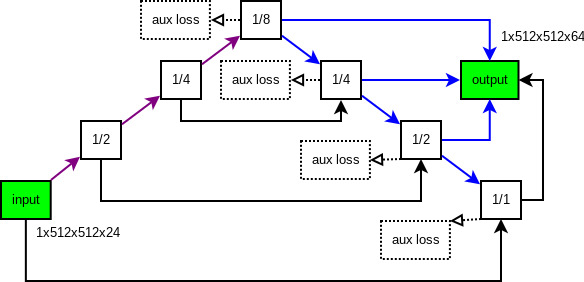
\includegraphics[width=\linewidth]{img/leaf/Diagram8.png}
        \tikzset{
	ppblock/.style={
		rectangle,
		minimum size=6mm,
		very thick,
		draw=black!50,
		text centered,
		font=\ttfamily,
		minimum width=8em,
		minimum height=6mm,
		top color=white,
	},
	%
	figure/.style={
		rectangle,
		rectangle split,
		rectangle split parts=2,
		very thick,
		draw=black!50,
		text centered,
		append after command={
			\pgfextra
			\fill[top color=#1, bottom color=#1]
			(\tikzlastnode.one west) 
			[rounded corners] |- (\tikzlastnode.north) -| (\tikzlastnode.one east) 
			[sharp corners]   |- (\tikzlastnode.one split) -| cycle;
			\fill[top color=white, bottom color=#1]
			(\tikzlastnode.two west) 
			[rounded corners] |- (\tikzlastnode.south) -| (\tikzlastnode.two east)  
			[sharp corners]   |- (\tikzlastnode.one split) -| cycle;
			\endpgfextra
		},
	},
    splitted/.style={
        rectangle,
        rectangle split,
        rectangle split horizontal,
        rectangle split parts=2,
        very thick,
        draw=black!50,
        text centered,
        append after command={
            \pgfextra
            \fill[top color=white, bottom color=#1]
            (\tikzlastnode.south)
            [rounded corners] -| (\tikzlastnode.west) |- (\tikzlastnode.one north)
            [sharp corners]   -| (\tikzlastnode.one split) |- cycle;
            \fill[top color=white, bottom color=#1]
            (\tikzlastnode.two south)
            [rounded corners] -| (\tikzlastnode.east) |- (\tikzlastnode.north)
            [sharp corners]   -| (\tikzlastnode.one split) |- cycle;
            \endpgfextra
        },
    },
	%
	static/.style={ppblock, bottom color={black!20}},
	nonterminal/.style={ppblock, bottom color={blue!30}},
	terminal/.style={ppblock, bottom color={green!20}},
	algorithm/.style={ppblock, bottom color={yellow!50}},
	error/.style={ppblock, bottom color={red!20}},
	type/.style={ppblock, bottom color={red!20}},
	loss/.style={ppblock, dashed, bottom color={black!20}, font=\itshape},
	%
	tiny/.style={
		rounded rectangle,
		very thick,
		draw=black!50,
		top color=white,
		bottom color=red!20,
        text centered,
		font=\ttfamily,
	},
    operator/.style = {
        circle,
        scale=0.6,
        draw=black!50,
        top color=white,
        bottom color=red!20,
        font=\boldmath,
    },
	%
	skip loop/.style={to path={-- ++(0,#1) -| (\tikztotarget)}}
}

\begin{tikzpicture}[
		>=stealth',thick,
		tip/.style={->,shorten >=0.007pt},
		every node/.style={scale=0.7},
		]
		\matrix[column sep=2mm, row sep=2mm, align=center] {
			\node (aux1)   [loss]      {Aux Loss};
			&  &  &
			\node (r181)[tiny]      {1/8};
			& & & & &
			\node (out)    [terminal]         {Output \\ 1x512x512x64};\\
			
			& &
			\node (r141)   [tiny]      {1/4}; & &
			\node (r142)   [tiny]      {1/4}; & & & &
			\node (aux2)   [loss]      {Aux Loss}; 
			& \\
			
			&
			\node (r121)   [tiny]      {1/2}; 
			& & & &
			\node (r122)   [tiny]      {1/2}; & & &
			\node (aux3)   [loss]      {Aux Loss};
			& \\
			
			\node (raw)    [terminal]      {Input \\ 1x512x512x24};
			& & & & & &
			\node (r111)   [tiny]   {1/1}; & &
			\node (aux4)   [loss]          {Aux Loss};
			\\
		};
		
		
		\begin{scope}[->,rounded corners=2mm]
		\draw[->, purple]     (raw.north) to [in=180,out=90] (r121.west);
		\draw[->, purple]     (r121.north) to [in=180,out=90] (r141.west);
		\draw[->, purple]     (r141.north) to [in=180,out=90] (r181.west);
		
		\draw[->]     (r141) to (r142);
		\draw[->]     (r121) to (r122);
		\draw[->]     (raw) to (r111);
		
		\draw[->, blue]     (r181.east) to [out=0,in=90] (r142.north);
		\draw[->, blue]     (r142.east) to [out=0,in=90] (r122.north);
		\draw[->, blue]     (r122.east) to [out=0,in=90] (r111.north);
		
		\draw[->, blue]     (r181.east) -- (out.west);
		\draw[->, blue]     (r142.east) |- (out.west);
		\draw[->, blue]     (r122.east) |- (out.west);
		\draw[->, blue]     (r111.east) |- (out.west);
		
		\draw[->, dashed]     (r181) -- (aux1);
		\draw[->, dashed]     (r142) -- (aux2);
		\draw[->, dashed]     (r122) -- (aux3);
		\draw[->, dashed]     (r111) -- (aux4);
		\end{scope}
		
		\end{tikzpicture}
		\\
        \caption{Synthesis of the core network based on MFP-Unet.Red arrows shows MaxPooling. Blue arrows shows Conv+UpSampling. Black arrows shows Conv. Sub-scale ratio are labelled on corresponding layer. The final output is the concatenation of features UpSampling. Multiple arrows shows concatenation as input layer}
        \label{fig:07-mfp-unet}
    \end{figure}
    \subsubsection{Downstream of the network} %! ce n'est ni du pre-processing, ni du post-rocessing
    It is composed of three \textbf{downstream} modules: CoordConv and Universal  Function  Approximator  (UFA) and Classification.
    \paragraph{CoordConv} The core network model produces a concatenation of 4 layers of 16 features ($4 \times 512 \times 512 \times 16$) which results of a layer of size $1 \times 512 \times 512 \times 64$. A coordinate layer \cite{liu2018intriguing} is also concatenated and allows to consider the mapping between the coordinates in (x,y) Cartesian space to one-hot pixel space. Three variables are appended, the normalized $x$ and $y$ coordinate and the radial coordinate $\sqrt{(x-0.5)^2+(y-0.5)^2}$. This module improves the results removing noise, ground moisture and it fixes few small holes in the segmentation mask.
    
    \paragraph{Universal Function Approximator (UFA)} This UFA -- also presented on the upstream -- is used to accurately mix features coming from various scales as well as the Cartesian coords. This module reconstructs the mapping function from the Cartesian space to a spatio-spectral feature of size $1 \times 512 \times 512 \times 16$. However, in contrast with the upstream UFA, the kernel size $k$ was fixed to $3$ to take into account neighboring.
    
    \paragraph{Classification and Auxiliary output}
    
    The classification is done through a small network composed of two $1\times1$ convolution layers. Followed by a ``Pyramid Pooling Module'' to consider different scales before the outputs and smooth the boundary prediction. \cite{zhao2017pyramid} showed that fusing the low to high-level features improved the segmentation task. It consists in the sum of different 2D convolutions whose kernel sizes have been set to 3, 5, 7 and 9. The number of filters is the same as the number of classes : $4$ (defined in \ref{sec:proposed-cnn}). The result of each convolution is concatenated and the final image output is given by a 2D convolution. In addition all convolutions are followed by a Batch Normalization and a sigmoid activation function. The figure \ref{fig:07-diagram2} shows that sub-network.
    
    \begin{figure}[H]
        \centering
        %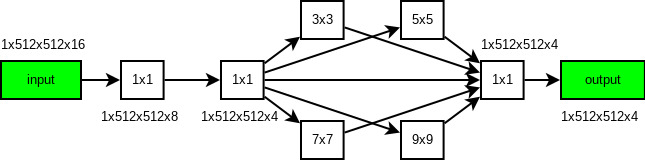
\includegraphics[width=\linewidth]{img/leaf/Diagram2} \\
        \tikzset{
	ppblock/.style={
		rectangle,
		minimum size=6mm,
		very thick,
		draw=black!50,
		text centered,
		font=\ttfamily,
		minimum width=8em,
		minimum height=6mm,
		top color=white,
	},
	%
	figure/.style={
		rectangle,
		rectangle split,
		rectangle split parts=2,
		very thick,
		draw=black!50,
		text centered,
		append after command={
			\pgfextra
			\fill[top color=#1, bottom color=#1]
			(\tikzlastnode.one west) 
			[rounded corners] |- (\tikzlastnode.north) -| (\tikzlastnode.one east) 
			[sharp corners]   |- (\tikzlastnode.one split) -| cycle;
			\fill[top color=white, bottom color=#1]
			(\tikzlastnode.two west) 
			[rounded corners] |- (\tikzlastnode.south) -| (\tikzlastnode.two east)  
			[sharp corners]   |- (\tikzlastnode.one split) -| cycle;
			\endpgfextra
		},
	},
    splitted/.style={
        rectangle,
        rectangle split,
        rectangle split horizontal,
        rectangle split parts=2,
        very thick,
        draw=black!50,
        text centered,
        append after command={
            \pgfextra
            \fill[top color=white, bottom color=#1]
            (\tikzlastnode.south)
            [rounded corners] -| (\tikzlastnode.west) |- (\tikzlastnode.one north)
            [sharp corners]   -| (\tikzlastnode.one split) |- cycle;
            \fill[top color=white, bottom color=#1]
            (\tikzlastnode.two south)
            [rounded corners] -| (\tikzlastnode.east) |- (\tikzlastnode.north)
            [sharp corners]   -| (\tikzlastnode.one split) |- cycle;
            \endpgfextra
        },
    },
	%
	static/.style={ppblock, bottom color={black!20}},
	nonterminal/.style={ppblock, bottom color={blue!30}},
	terminal/.style={ppblock, bottom color={green!20}},
	algorithm/.style={ppblock, bottom color={yellow!50}},
	error/.style={ppblock, bottom color={red!20}},
	type/.style={ppblock, bottom color={red!20}},
	loss/.style={ppblock, dashed, bottom color={black!20}, font=\itshape},
	%
	tiny/.style={
		rounded rectangle,
		very thick,
		draw=black!50,
		top color=white,
		bottom color=red!20,
        text centered,
		font=\ttfamily,
	},
    operator/.style = {
        circle,
        scale=0.6,
        draw=black!50,
        top color=white,
        bottom color=red!20,
        font=\boldmath,
    },
	%
	skip loop/.style={to path={-- ++(0,#1) -| (\tikztotarget)}}
}

\vspace{-1em}
\begin{tikzpicture}[
		>=stealth',thick,
		tip/.style={->,shorten >=0.007pt},
		every node/.style={scale=0.7},
		]
		\matrix[column sep=4mm, row sep=2mm, align=center] {
			
			\node (raw)    [terminal]      {Input \\ 1x512x512x16}; &
			\node (conv1)  [nonterminal]   {Conv 1x1 \\ 1x512x512x8};
			&&
			\node (conv3)  [nonterminal, minimum width=4em]   {Conv 3x3}; &
			\node (conv4)  [nonterminal, minimum width=4em]   {Conv 5x5}; \\
			
			&\node (conv2)  [nonterminal]   {Conv 1x1 \\ 1x512x512x4};      &
			& & &
			\node (conv7)  [nonterminal]   {Conv 1x1 \\ 1x512x512x4};    \\
			
			
			&&&
			\node (conv5)  [nonterminal, minimum width=4em]   {Conv 7x7}; &
			\node (conv6)  [nonterminal, minimum width=4em]   {Conv 9x9}; &
			\node (out)    [terminal]      {Output \\ 1x512x512x4};        \\
		};
		
		
		\begin{scope}[->,rounded corners=2mm]
		\draw[->]     (raw) to (conv1);
		\draw[->]     (conv1) to (conv2);
		
		\draw[->]     (conv2.east) to (conv3.west);
		\draw[->]     (conv2.east) to (conv4.south west);
		\draw[->]     (conv2.east) to (conv5.west);
		\draw[->]     (conv2.east) to (conv6.north west);
		\draw[->]     (conv2.east) to (conv7);
		
		\draw[->]     (conv3.south) to [in=180, out=-90,looseness=0.5] (conv7.west);
		\draw[->]     (conv4.south) to [in=180, out=-90] (conv7.west);
		\draw[->]     (conv5.north) to [in=180, out=90,looseness=0.5] (conv7.west);
		\draw[->]     (conv6.north) to [in=180, out=90] (conv7.west);
		
		\draw[->]     (conv7) to (out);
		
		\end{scope}
		
\end{tikzpicture}\\
        \caption{Auxiliary output and classification module. Multiple arrows shows concatenation as input layer}
        \label{fig:07-diagram2}
    \end{figure}
    
    \subsection{Loss function}
    \label{sec:loss-function}
    
    A wide variety of loss functions have been developed during the emergence of deep-learning. Recently, \cite{MIoU2016} proposed a solution to optimize an approximation of the mean Intersection over Union (mIoU) which seems to be optimal for binary segmentation \cite{zhou2019iou}. The loss function using ground truth ($p$) and the prediction ($\hat{p}$) is defined by:
    \begin{equation} \texttt{mIoU}(p, \hat{p}) = 1 - \frac{p\hat{p}}{p+\hat{p} - p\hat{p}} \end{equation}
    
    This loss function was used on each auxiliary. In addition the loss is computed separately on each class, weighted (denoted $W_C$) and summed. The result of this function is:
    \begin{equation} \texttt{Aux}(p, \hat{p}) = \sum_{C=0}^{4} W_C \times \texttt{mIoU}(p_C, \hat{p}_C) \end{equation}
    
    % x = np.array([1,3,1.2,0.5])
    % x/np.sum(x)
    
    In the above equation, the weight $W$ were empirically set to $[0.175, 0.526, 0.211, 0.09]$. Meaning that the second class (inner edges) is prioritized (to separate inner instance). Then it is outer edges that allow to separate the ``big'' leaves from small or thin leaves. Finally the thin leaves (mostly spectral mixing) and inner big leaves (essentially vegetation minus boundaries) have the smallest weight values because these classes should be easier to learn.
    
    In recent CNN architectures for instance segmentation, the loss function does not take into account the number of detected instances or the shape of the segmentation. This aspect is only evaluated after learning, e.g., using a symmetric best dice metric. This implies that we can not guaranty that the network is well learned on crowded scene, where instance is generally merged. One problem is that until recently, instances could not be retrieved directly during the learning phase, this is due to the ``non-maximal suppression'' algorithm required after the CNN or the time required for the association between the detected instances and the ground truth. In this paper, we introduce a new loss function considered at the downstream of the network. The main idea is to take into account an approximation of the segmentation quality of each leaf.
    To estimate the segmentation quality, the undetected, under/over segmented and fused objects can be evaluated, trough a sorted histogram of the number of pixels associated to each connected component for both prediction and ground truth, as showed in the next figure \ref{fig:07-loss} for both prediction (orange) and ground truth (blue).
    
    \begin{figure}[H]
        \centering
        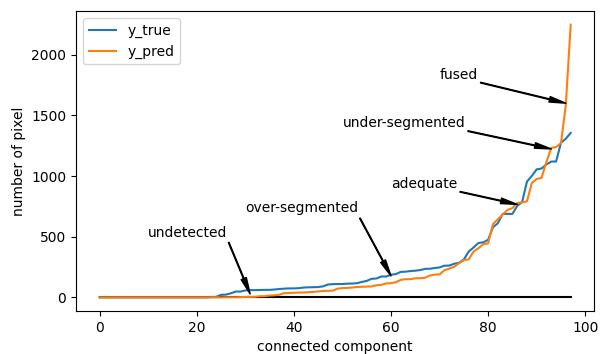
\includegraphics[width=0.7\linewidth]{img/leaf/Loss}
        \caption{Sorted histogram of the number of pixels associated to each component, the blue (resp. red) line represents the true (resp. predicted) number of pixels for each component.}
        \label{fig:07-loss}
    \end{figure}
    
    This figure shows that when the prediction curve is lower (orange) than the ground truth curve (blue), it means that there is over-segmentation. This arise when a bigger element is split in two, when the borders of the shape are trimmed or when zero pixels of the shape are detected (undetected). On the other hand, when the prediction curve is higher than the ground truth, it means that the contours of the shape are roughly detected or if it greatly exceeds the ground truth, then we are in the presence of fused shapes. Based on these curves, a loss function can be construct the deal with over and under segmentation on shape criterion, thus a custom absolute percentage error was defined:
    
    \begin{eqnarray}
    \texttt{Leaf}(p, \hat{p}) = \frac{\sum_{i=0}^{N} |\texttt{leaky\_relu}(h_i(p)-h_i(\hat{p}))| }{h_{max}(p)+1} \\
    \texttt{leaky\_relu}(x) =
    \begin{cases}
    \mbox{$x$} & \mbox{if } x >= 0\\
    \mbox{$x*0.2$} & \mbox{if } x < 0
    \end{cases}
    \end{eqnarray}
    
    On the above equation $N$ is the number of components, $h_i(p)$, and $h_i(\hat{p})$ is respectively the number of pixels of a connected component in the ground truth and on the predicted segmentation within the sorted histogram. While $h_{max}(p)$ is the maximum number of pixels of a component in the ground truth.
    
    \newpage
    The leaky\_relu, is used to explicitly prioritise the learning on under-segmentation rather than over-segmentation which allows to prioritize the merged objects. This was defined because conventional losses did not give good results in dense vegetation cover, causing a large segmented area that is detected as a single entity. Note also that over-segmentation is less problematic, since it occurs mainly around the borders of the leaves, which are recovered later, through a watershed algorithm (section \ref{sec:watershed-refinement}). It is the first study to suggest this type of loss.
    
    The downstream loss is defined by $\texttt{DownAux}(p, \hat{p}) = \texttt{Aux}(p, \hat{p}) + \texttt{Leaf}(p, \hat{p})$. Finally the global loss considers the upstream auxiliary loss, each of the 4 feature scale auxiliary loss and the downstream loss. Thus the global loss is defined as the weighted sum of all auxiliaries losses (in the same order) where the weights $W$ were empirically defined with $W = [0.01, 1.0, 0.1, 0.1, 0.01, 4.0]$.
    
    \subsection{Refinement with vegetation mask and watershed}
    \label{sec:watershed-refinement}
    
    
    The used U-Net architecture is good at detecting ``big'' elements on the scene but lacks precision on very small and thin elements.  A method to produce an optimized vegetation mask was proposed in  a previous work  \cite{Vayssade2021}. Using this mask provides better performance than adding a specific class to the network. Thus our previous work is used here to get the best foreground/background segmentation mask as input of the watershed. It is also learned on a specific dataset with more illumination conditions and should be more robust, especially for thin elements.
    
    The proposed network generates 4 classes. The first two are associated to ``big'' leaf boundaries (denoted $Edges=Outer+Inner$). The third one is small and thin leaves (denoted $Thin$), and the fourth is the inner of big leaves denoted $Big$. The watershed seed is defined with the following equation \ref{eq:watershed-seed} to generate the seed mask and can be see in the figure \ref{fig:07-refined-watershed} :
    
    \begin{equation}
    Seed = Thin + Big - Edges
    \label{eq:watershed-seed}
    \end{equation}
    
    \begin{figure}[H]
        \centering
        \vspace{-1em}
        %\includegraphics[width=\linewidth]{img/leaf/refined-watershed-2.png}
        \tikzset{
	ppblock/.style={
		rectangle,
		minimum size=6mm,
		very thick,
		draw=black!50,
		text centered,
		font=\ttfamily,
		minimum width=8em,
		minimum height=6mm,
		top color=white,
	},
	%
	figure/.style={
		rectangle,
		rectangle split,
		rectangle split parts=2,
		very thick,
		draw=black!50,
		text centered,
		append after command={
			\pgfextra
			\fill[top color=#1, bottom color=#1]
			(\tikzlastnode.one west) 
			[rounded corners] |- (\tikzlastnode.north) -| (\tikzlastnode.one east) 
			[sharp corners]   |- (\tikzlastnode.one split) -| cycle;
			\fill[top color=white, bottom color=#1]
			(\tikzlastnode.two west) 
			[rounded corners] |- (\tikzlastnode.south) -| (\tikzlastnode.two east)  
			[sharp corners]   |- (\tikzlastnode.one split) -| cycle;
			\endpgfextra
		},
	},
    splitted/.style={
        rectangle,
        rectangle split,
        rectangle split horizontal,
        rectangle split parts=2,
        very thick,
        draw=black!50,
        text centered,
        append after command={
            \pgfextra
            \fill[top color=white, bottom color=#1]
            (\tikzlastnode.south)
            [rounded corners] -| (\tikzlastnode.west) |- (\tikzlastnode.one north)
            [sharp corners]   -| (\tikzlastnode.one split) |- cycle;
            \fill[top color=white, bottom color=#1]
            (\tikzlastnode.two south)
            [rounded corners] -| (\tikzlastnode.east) |- (\tikzlastnode.north)
            [sharp corners]   -| (\tikzlastnode.one split) |- cycle;
            \endpgfextra
        },
    },
	%
	static/.style={ppblock, bottom color={black!20}},
	nonterminal/.style={ppblock, bottom color={blue!30}},
	terminal/.style={ppblock, bottom color={green!20}},
	algorithm/.style={ppblock, bottom color={yellow!50}},
	error/.style={ppblock, bottom color={red!20}},
	type/.style={ppblock, bottom color={red!20}},
	loss/.style={ppblock, dashed, bottom color={black!20}, font=\itshape},
	%
	tiny/.style={
		rounded rectangle,
		very thick,
		draw=black!50,
		top color=white,
		bottom color=red!20,
        text centered,
		font=\ttfamily,
	},
    operator/.style = {
        circle,
        scale=0.6,
        draw=black!50,
        top color=white,
        bottom color=red!20,
        font=\boldmath,
    },
	%
	skip loop/.style={to path={-- ++(0,#1) -| (\tikztotarget)}}
}

\begin{tikzpicture}[
        >=stealth',thick,
        tip/.style={->,shorten >=0.007pt},
        every node/.style={scale=0.7},
    ]
    
    \matrix (table) [matrix of nodes, column sep=6mm, row sep=6mm, align=center] {
        \node (false)        [figure={green!20}]      {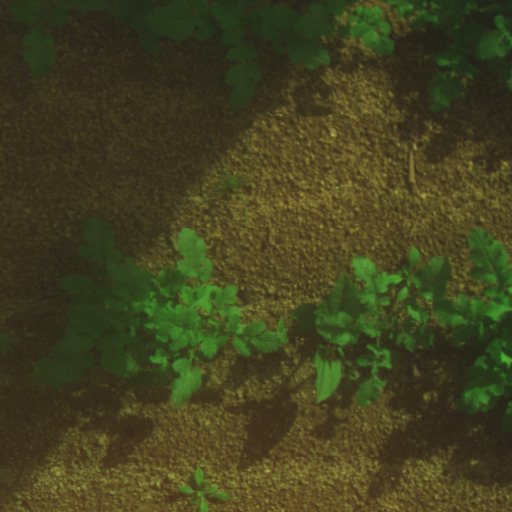
\includegraphics[width=4cm]{img/leaf/airphen-false} \nodepart{second} \large Input Image}; &
        \node (detection)    [figure={blue!30}]      {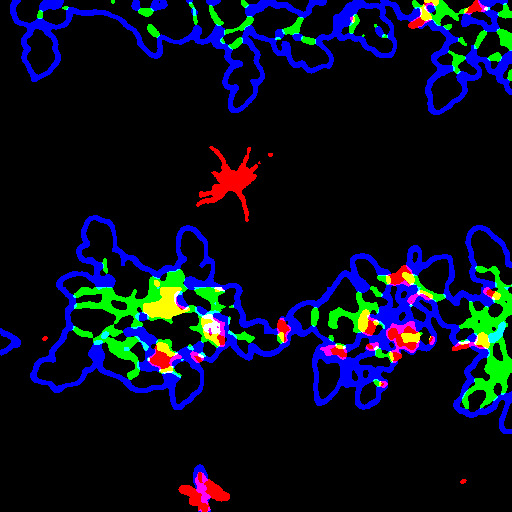
\includegraphics[width=4cm]{img/leaf/airphen-detection} \nodepart{second} \large CNN Outputs}; &
        \node (body)         [figure={blue!30}]      {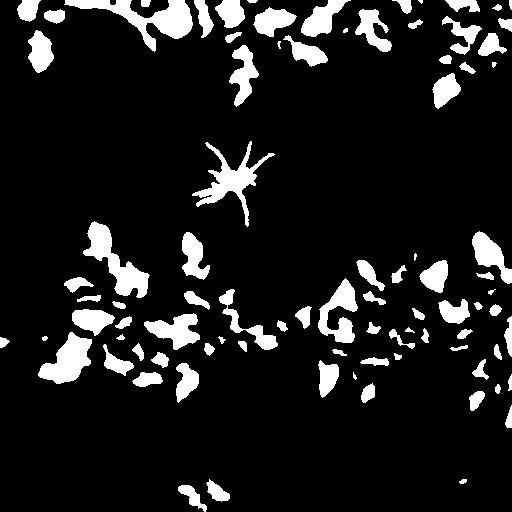
\includegraphics[width=4cm]{img/leaf/airphen-body} \nodepart{second} \large Watershed Seeds}; \\
        
        &
        \node (index)        [figure={black!20}]      {\includegraphics[width=4cm]{img/leaf/airphen-index} \nodepart{second} \large Deep-Indices}; &
        \node (watershed)    [figure={green!20}]      {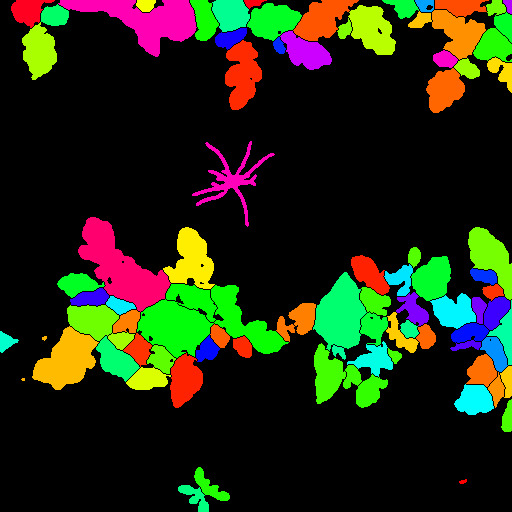
\includegraphics[width=4cm]{img/leaf/airphen-watershed} \nodepart{second} \large Refined Ouput}; \\
    };
    
    \draw[->] (false) to (detection);
    \draw[->] (detection) to (body);
    \draw[->] (body) to (watershed);
    \draw[->] (index) to (watershed);
    \draw[->] (false) |- (index);
    
\end{tikzpicture}
        \caption{The refinement of the CNN output through watershed and Deep-Indices. The Seed of the equation \ref{eq:watershed-seed} can be seen on the ``watershed seed'' image.}
        \label{fig:07-refined-watershed}
    \end{figure}
    
    \subsection{Training setup}
    
    The image dataset is randomly split into a training set (80\%) and a validation set (20\%). However the initial seed is kept for reproducibility. In addition a random data augmentation is used during the training to increase the dataset variability. A random vertical and horizontal flip is considered as well as a perlin simplex noise \cite{perlin_noise} (of size $512 \times 512$), set with 2 modal in range $[0.7-1.3]$ which multiplies the number of input images. Low values add shadows, while high values add specular effects. The training is done through Keras module within Tensorflow 2.6.0 framework. All computations are done on an NVidia RTX 3060 which have 12GiB of memory and due to the size of the network only one image is computed at once.
    
    \subsection{Evaluation metrics}
    
    There is a large number of possible evaluation metrics for instance segmentation, which have been reviewed in \cite{scharr2016leaf}. However, we decided to keep the evaluation metrics used in the Leaf Segmentation Challenge (LSC) as a reference for comparison \cite{scharr2017computer, kulikov2018instance, bell2019leaf, ward2020scalable}. Therefore, we use the foreground/background DICE metric to evaluate the separation of large leaves from the ground (denoted $FgBgDice$). We estimate the average accuracy of leaf segmentation by the symmetric best DICE score among all objects (leaves). The best DICE score among all objects (leaves) to estimate the average accuracy of leaf segmentation is denoted $BestDice$. The $AbsDiffFG$  estimates how good the algorithm is at segmenting the leaves. And finally, $DiffFG$ estimates the efficiency of the algorithm for counting  leaves.
    $SBD$ for Symmetric best DICE is extract to estimate the average leaf segmentation accuracy.
    All these metrics are common and presented by \cite{scharr2016leaf}.
    In addition, to compare datasets results, a new metric is introduced named $NAbsDiffFG$ defined by the division of $AbsDiffFG$ and the mean of leaves count in the dataset.
    
    \section{Results}
    
    As previously defined, all datasets were split into training and validation sets with a ratio of $80-20\%$. Once training is done on the defined setup and using the loss function, the evaluation metrics are extracted :
    the $FGBGDice$ metric is used to evaluate the soil versus vegetation segmentation, while the $BestDice$ metric is used to evaluate the instance segmentation. Each connected component is associated to its best corresponding ground truth based on a dice score. Then the metric is defined by the mean dice score of the best match. Other metrics show relevant information about over and under segmentation. The following subsections are dedicated to each dataset, from the simplest to the most difficult to segment.
    
    \subsection{Komatsuna dataset}
    
    The first one is the Komatsuna dataset. It is composed of RGB data of growing Japanese Mustard. This dataset is interesting for its controlled illumination conditions. In addition, the number of leaves it quite the same for all the growing stages, ranging from 3 to 6 leaves. This is important regarding our loss function which take into account the quantity and quality of each segmented leaf. However, this dataset  does not contain small and thin leaves, thus the third class was replaced by a foreground class. The following Table \ref{tab:eval-komatsuna} shows the evaluation on this dataset.
    
    \newpage
    \null
    \vfill
    \begin{table}[H]
        \rowcolors{0}{gray!10}{white}
        \begin{tabularx}{\linewidth}{|X|r|r|}
            \hline
            \textbf{Metric} 				& \textbf{Training} &  \textbf{Validation}  \\ \hline
            FgBgDice 			&   0.9732 &   0.9715 \\
            BestDice 			&   0.8796 &   0.8565 \\
            SBD 	            &   0.8713 &   0.8517 \\
            DiffFG 		        &  -0.2639 &  -0.4444 \\
            AbsDiffFG 	        &   0.3944 &   0.5222 \\ \hline
            Number of images 	&      720 &      180 \\
            Mean leaf count 	&   4.9194 &   4.9722 \\
            NAbsDiffFG          &   0.0802 &   0.1050 \\
            \hline
        \end{tabularx}
        \caption{Evaluation metrics for the Komatsuna dataset}
        \label{tab:eval-komatsuna}
    \end{table}
    \vfill
    
    The result on this dataset shows a relatively perfect score of the soil and vegetation segmentation with a $FGBGDice$ of 0.97. Few errors remain as shown in figure \ref{fig:07-eval-komatsuna}, a green bottle is visible on the left side of some images, which seems to indicate that the green component has a major impact on vegetation detection. Since RGB data are used, this error should be visible in most studies. This interesting element also demonstrate that the used \textit{CoordConv} layer does not play its role in the spatial management of this element.
    
    \vfill
    \begin{figure}[H]
        \centering
        \FramedBox{.5cm}{0.3\linewidth}{Input}
        \FramedBox{.5cm}{0.3\linewidth}{CNN output}
        \FramedBox{.5cm}{0.3\linewidth}{Ground truth} \\
        
        \FramedBox{0.3\linewidth}{0.3\linewidth}{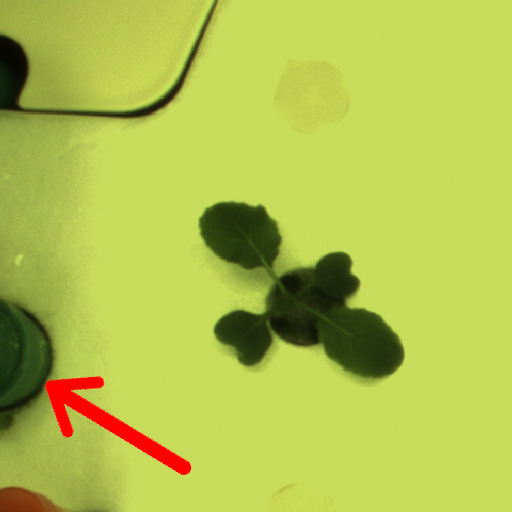
\includegraphics[width=\linewidth]{img/leaf/results-komatsuna-0}}
        \FramedBox{0.3\linewidth}{0.3\linewidth}{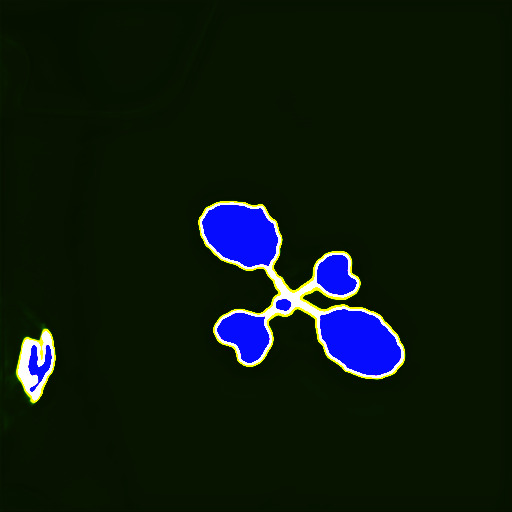
\includegraphics[width=\linewidth]{img/leaf/results-komatsuna-1}}
        \FramedBox{0.3\linewidth}{0.3\linewidth}{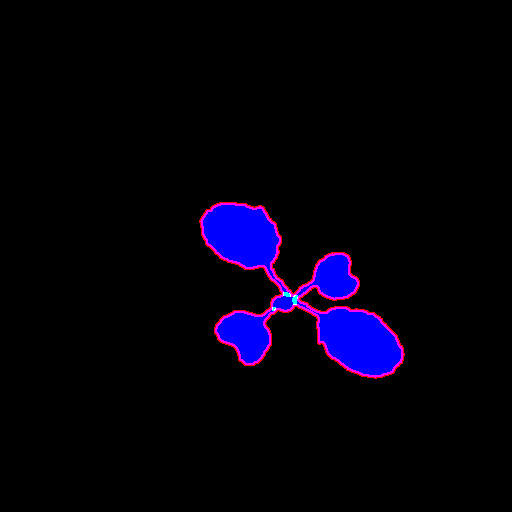
\includegraphics[width=\linewidth]{img/leaf/results-komatsuna-7}} \\
        
        \UnframedBox{0.3\linewidth}{0.3\linewidth}{
\includegraphics[width=\linewidth]{img/leaf/empty}}
        \FramedBox{0.3\linewidth}{0.3\linewidth}{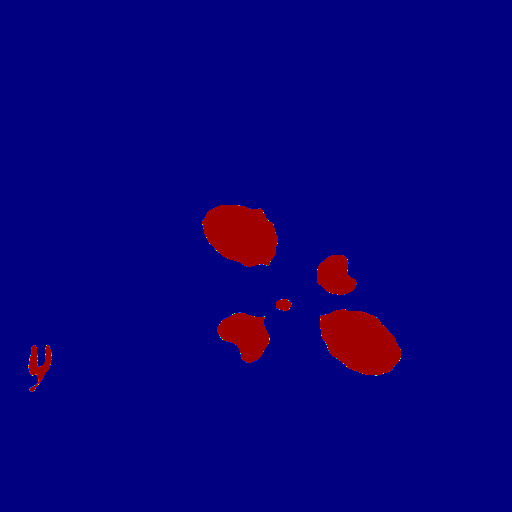
\includegraphics[width=\linewidth]{img/leaf/results-komatsuna-2}}
        \FramedBox{0.3\linewidth}{0.3\linewidth}{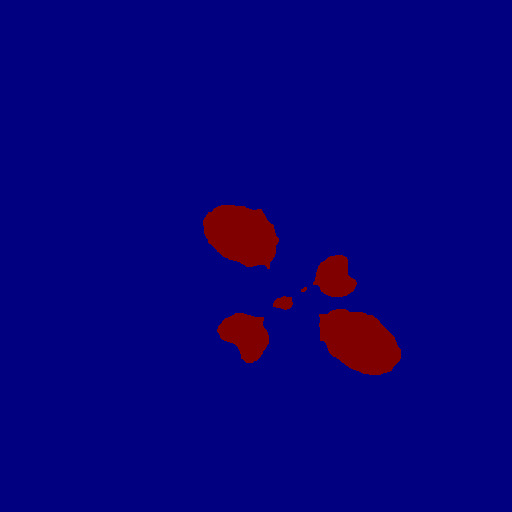
\includegraphics[width=\linewidth]{img/leaf/results-komatsuna-8}} \\
        
        \caption{Visual comparison of Komatsuna dataset after the training, the red arrow in the input image shows a green bottle}
        \label{fig:07-eval-komatsuna}
    \end{figure}
    \vfill
    \null

    \newpage
    As shown by the $DiffFG$ score, our method mostly detects the right number of leaves. This score is small and negative and shows that few leaves are split, which occurs when a big leaf mostly overlaps a smaller one.
    A visible bottle also has an impact on the other metrics, shown in figure \ref{fig:07-eval-komatsuna}. However, most of the errors for the $BestDice$ comes from under and over-segmentation. The under-segmentation occurs on the leaves stems. The stem that connects the leaf to the plant is usually not well detected, and this can play a significant role in lowering the $BestDice$ and $SymmetricBestDice$ scores. The stem can be undetected (under-segmentation) or may be identified as another leaf (over-segmentation). It can also cover some small leaves and divide them in two, which is expected in pixelwise segmentation.  To benchmark our study, the following table \ref{tab:komatsuna-detectron} reports the results of few previous studies using the same metrics.
    
    \begin{table}[H]
        \centering
        \rowcolors{0}{gray!10}{white}
        \begin{tabularx}{\linewidth}{|X|r|r|}
            \hline
            \textbf{Study}                                       & \textbf{SBD} & \textbf{AbsDiffFG} \\ \hline
            Our method's results (2021)                & \textbf{0.8565} & \textbf{0.5222} \\
            \cite{ward2020scalable}      ward 2020      & 0.7776 &   -    \\
            \cite{gomes2020leaf}         gomes 2020     & 0.7700 & 0.8800 \\
            \hline
        \end{tabularx}
        \caption{Comparison of the ResNet 101 based on Detectron II framework of facebook and the UPGen based on Mask-RCNN. Our solution is the most effective in both metrics}
        \label{tab:komatsuna-detectron}
    \end{table}
    As comparison our results tackle one of the states of the art ResNet 101 based on Detectron II framework of facebook \cite{gomes2020leaf}. And the proposed UPGen methods proposed by \cite{ward2020scalable}.
    
    \subsection{Leaf Segmentation Challenge dataset}
    
    The second dataset is interesting for its controlled illumination conditions. Unlike the Komatsuna dataset, this one includes a greater diversity of leaf quantity, between 2 and 16 leaves. This is important to show the robustness of our loss function.
    In the same regard as the Komatsuna section, this dataset does not contain small and thin leaves. Thus third class was replaced by a foreground class, which is also used by the competition evaluation. In addition, the testing dataset is not publicly available, thus a separated evaluation was performed on the online competition website \footnote{\url{competitions.codalab.org/competitions/18405}}. The training and validation are defined by splitting the publicly available dataset. This step is used to reduce the over-fitting and retrieve stable parameters. The next table summarizes the number of images for each training, validation and test datasets.
    
    \begin{table}[H]
        \centering
        \rowcolors{0}{gray!10}{white}
        \begin{tabularx}{\linewidth}{|X|r|r|r|r|r|r|}
            \hline
            \textbf{Dataset} 	 &  A1  &  A2 &   A3 &  A4 & \textbf{Total} \\ \hline
            \textbf{Training}    & 102  &  25 &   22 & 499 & 648 \\
            \textbf{Validation}  &  25  &   6 &    5 & 125 & 161 \\
            \textbf{Test}        &  33  &   9 &   56 & 168 & 266 \\
            %image size  & 530  & 565 & 2048 & 441 \\
            \hline
        \end{tabularx}
        \caption{Number of images for each sub LSC dataset}
        \label{tab:quantity-cvppp}
    \end{table}
    
    \newpage
    The following Table \ref{tab:eval-cvppp} shows the overall evaluation on this dataset (merged A1, A2, A3, A4). The test results can be found in the online leader-board. The results are fairly the same between training, validation and test datasets in term of $FGBGDice$ and $BestDice$. However a notable divergence with the testing dataset for the others metrics is visible. The $DiffFG$, and $AbsDiffFG$ for training and validation indicate an over-segmentation, while the test dataset highlights an under-segmentation. This over-segmentation probably enhances the $SBD$ score while the $BestDice$ remains stable.
    
    \begin{table}[H]
        \rowcolors{0}{gray!10}{white}
        \begin{tabularx}{\linewidth}{|X|r|r|r|}
            \hline
            \textbf{Metric} 	& \textbf{Training} & \textbf{Validation} &  \textbf{Test}  \\ \hline
            FgBgDice 			&   0.9489 &   0.9522   & 0.9489 \\
            BestDice 			&   0.7659 &   0.7707   & 0.7608 \\
            SBD 	            &   0.7608 &   0.7655   & 0.8047 \\
            DiffFG 		        &  -1.9634 &  -2.1223   & 3.5628 \\
            AbsDiffFG 	        &   2.1707 &   2.3050   & 6.1257 \\ \hline
            Number of images 	&      648 &      161   & 266    \\
            Mean leaf count 	&  13.8390 &  13.1463   & -      \\
            NAbsDiffFG          &   0.1568 &  0.1753    & -      \\
            \hline
        \end{tabularx}
        \caption{Evaluation metrics of the overall LSC dataset}
        \label{tab:eval-cvppp}
    \end{table}
    
    As discussed in the materials and data section, this database is composed of four sub-databases with different cameras and plants. The learning was done independently on each of them, but they were merged for the presentation in the previous table. The test on the online evaluation platform returns the results for each of them, summarized in the table \ref{tab:eval-sub-cvppp}. First of all, the sub-datasets A2 and A3 contain a very small amount of images, respectively 25 and 22 for the training sets. Moreover the A3 dataset is composed of images of size $2048 \times 2048$ re-scaled to $512 \times 512$. This imply a huge loss of information, especially on the leaf boundaries. In addition, this A3 dataset contains hard shadows. These three factors explain most of the errors for this dataset. The quality, acquisition conditions, and plants of the other three data sets (A1, A2, A4) are similar. Only the background and the amount of images mainly changes, which is also reflected in the evaluation score. The figure \ref{fig:07-cvppp-a4} also shows unlabeled leaves in the center of the plant, moreover they are even defined as background.
    
    \begin{table}[H]
        \rowcolors{0}{gray!10}{white}
        \begin{tabularx}{\linewidth}{|X|r|r|r|r|r|}
            \hline
            \textbf{Metric} 	&    A1   &   A2   &     A3   &   A4   \\ \hline
            FGBGDice 			&  0.9641 & 0.9294 &   0.9692 & 0.9416 \\
            BestDice 			&  0.6905 & 0.6944 &   0.6783 & 0.7964 \\
            SBD 	            &  0.8047 & 0.7895 &   0.7317 & 0.8294 \\
            DiffFG 		        &  2.0909 & 1.7778 &  21.2857 & 0.0892 \\
            AbsDiffFG 	        &  3.0000 & 3.1111 &  14.9285 & 1.6250 \\
            \hline
        \end{tabularx}
        \caption{Evaluation metrics of the independent sub LSC dataset}
        \label{tab:eval-sub-cvppp}
    \end{table}
    
    For all sub-dataset the $FGBGDice$ score is slightly less than the Komatsuna dataset. Most pictures of the A1 present wide area of green moisture on the ground, visible on the Input inside the figure \ref{fig:07-cvppp-a1}. A2 contains few very small weeds and few small spots of moisture, but the performances of $FGBGDice$ is mainly due to the quantity of images for the learning, as showed by the figure \ref{fig:07-cvppp-a2} boundaries are miss-classified. For the same reason, it is also visible for the A3 dataset shown by the figure \ref{fig:07-cvppp-a3}. It's also important to notice that leaves from an outside plant are visible in few images and detected by the algorithm, however these leaves are unlabelled, resulting an over-segmentation.
    
    \newpage
    \null
    \vfill
    \begin{figure}[H]
        \centering
        \FramedBox{.5cm}{0.25\linewidth}{Input}
        \FramedBox{.5cm}{0.25\linewidth}{CNN output}
        \FramedBox{.5cm}{0.25\linewidth}{Ground truth} \\
        \FramedBox{0.25\linewidth}{0.25\linewidth}{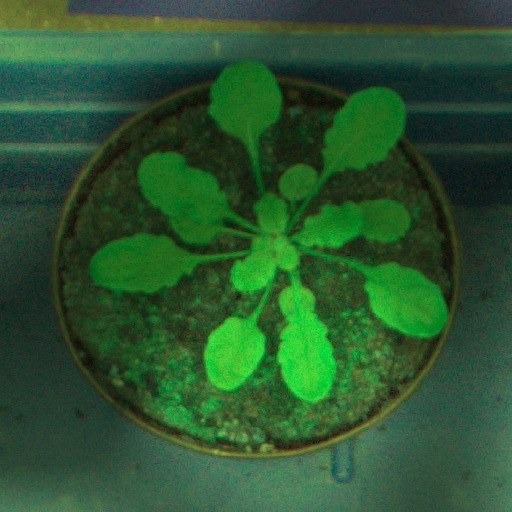
\includegraphics[width=\linewidth]{img/leaf/results-a1-0}}
        \FramedBox{0.25\linewidth}{0.25\linewidth}{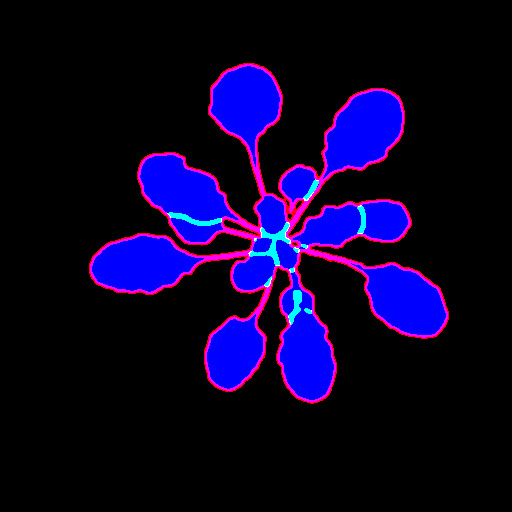
\includegraphics[width=\linewidth]{img/leaf/results-a1-1}}
        \FramedBox{0.25\linewidth}{0.25\linewidth}{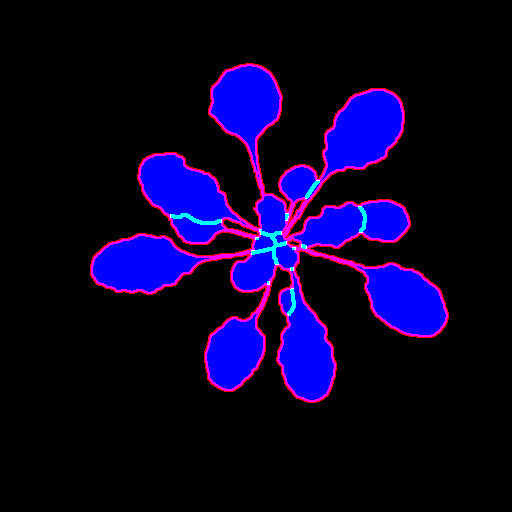
\includegraphics[width=\linewidth]{img/leaf/results-a1-7}} \\
        \UnframedBox{0.25\linewidth}{0.25\linewidth}{
\includegraphics[width=\linewidth]{img/leaf/empty}}
        \FramedBox{0.25\linewidth}{0.25\linewidth}{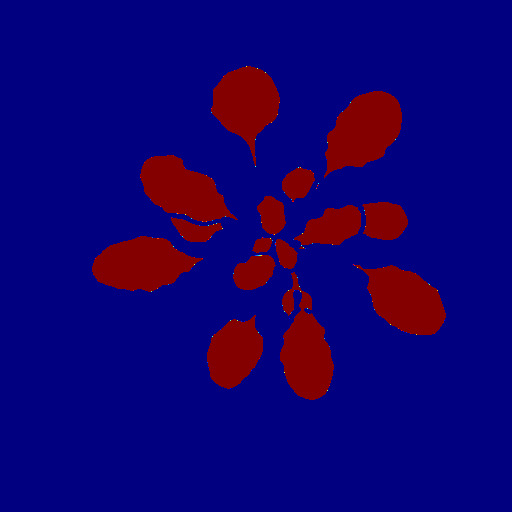
\includegraphics[width=\linewidth]{img/leaf/results-a1-2}}
        \FramedBox{0.25\linewidth}{0.25\linewidth}{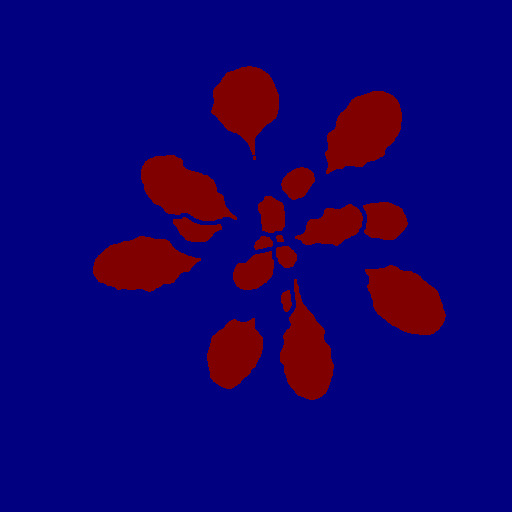
\includegraphics[width=\linewidth]{img/leaf/results-a1-8}} \\
        \caption{Visual example of LSC results for A1}
        \label{fig:07-cvppp-a1}
    \end{figure}
    \vfill
    \begin{figure}[H]
        \centering
        \FramedBox{.5cm}{0.25\linewidth}{Input}
        \FramedBox{.5cm}{0.25\linewidth}{CNN output}
        \FramedBox{.5cm}{0.25\linewidth}{Ground truth} \\
        \FramedBox{0.25\linewidth}{0.25\linewidth}{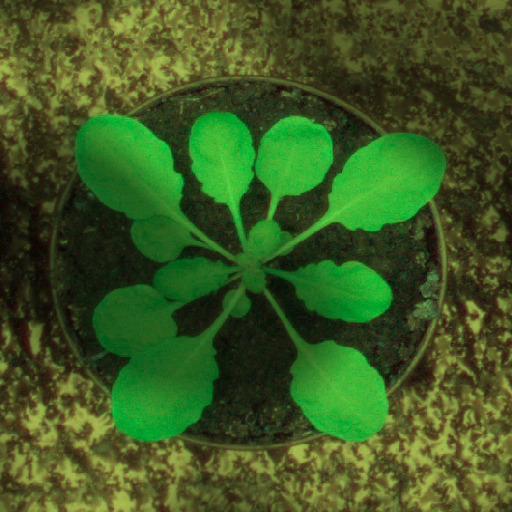
\includegraphics[width=\linewidth]{img/leaf/results-a2-0}}
        \FramedBox{0.25\linewidth}{0.25\linewidth}{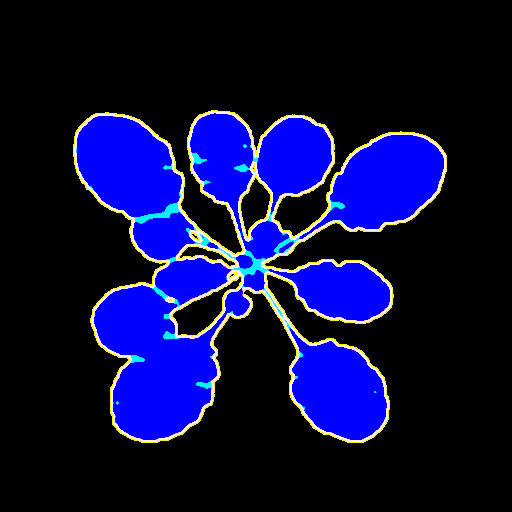
\includegraphics[width=\linewidth]{img/leaf/results-a2-1}}
        \FramedBox{0.25\linewidth}{0.25\linewidth}{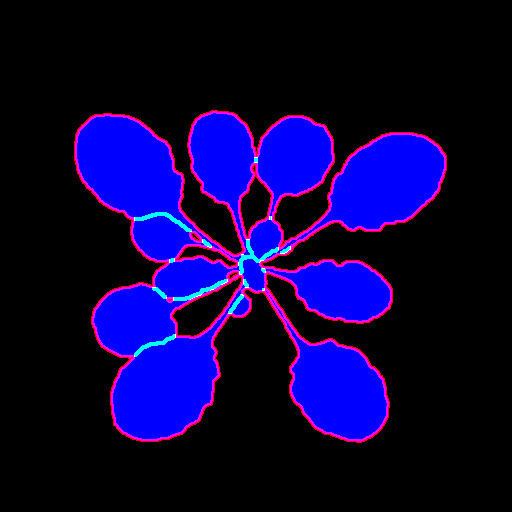
\includegraphics[width=\linewidth]{img/leaf/results-a2-7}} \\
        \UnframedBox{0.25\linewidth}{0.25\linewidth}{
\includegraphics[width=\linewidth]{img/leaf/empty}}
        \FramedBox{0.25\linewidth}{0.25\linewidth}{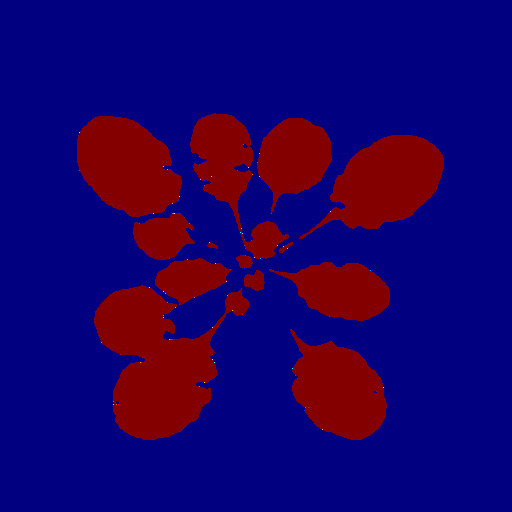
\includegraphics[width=\linewidth]{img/leaf/results-a2-2}}
        \FramedBox{0.25\linewidth}{0.25\linewidth}{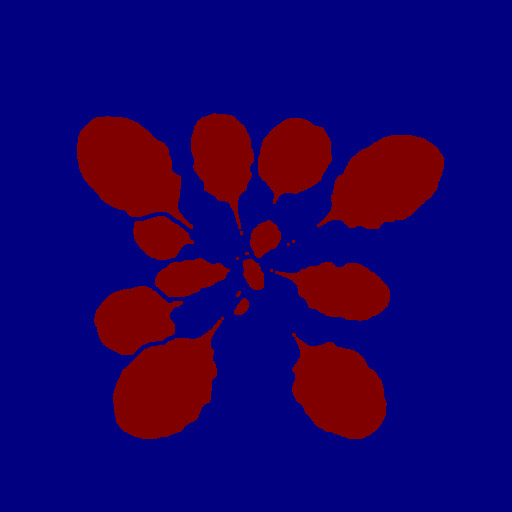
\includegraphics[width=\linewidth]{img/leaf/results-a2-8}} \\
        \caption{Visual example of LSC results for A2}
        \label{fig:07-cvppp-a2}
    \end{figure}
    \vfill
    
    
    \newpage
    \null
    \vfill
    \begin{figure}[H]
        \centering
        \FramedBox{.5cm}{0.25\linewidth}{Input}
        \FramedBox{.5cm}{0.25\linewidth}{CNN output}
        \FramedBox{.5cm}{0.25\linewidth}{Ground truth} \\
        \FramedBox{0.25\linewidth}{0.25\linewidth}{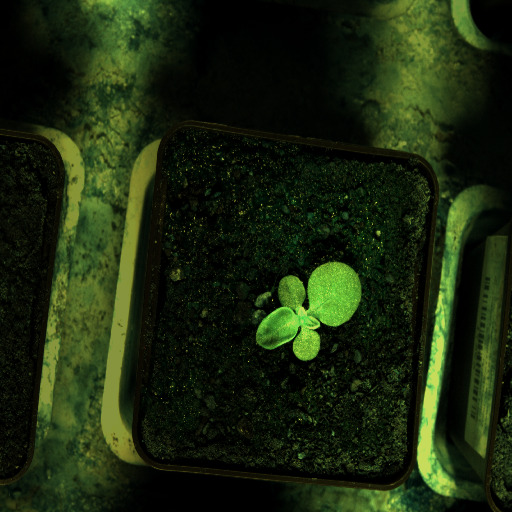
\includegraphics[width=\linewidth]{img/leaf/results-a3-0}}
        \FramedBox{0.25\linewidth}{0.25\linewidth}{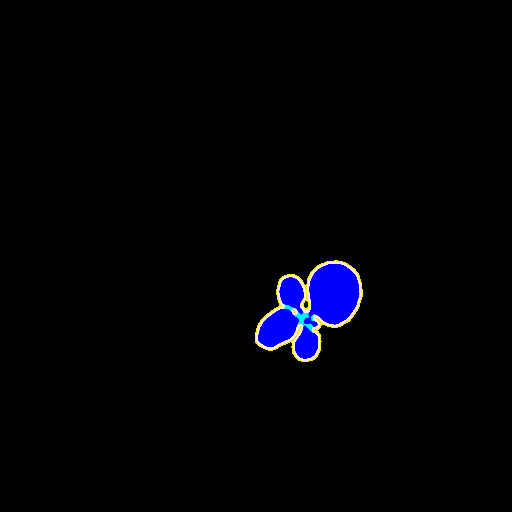
\includegraphics[width=\linewidth]{img/leaf/results-a3-1}}
        \FramedBox{0.25\linewidth}{0.25\linewidth}{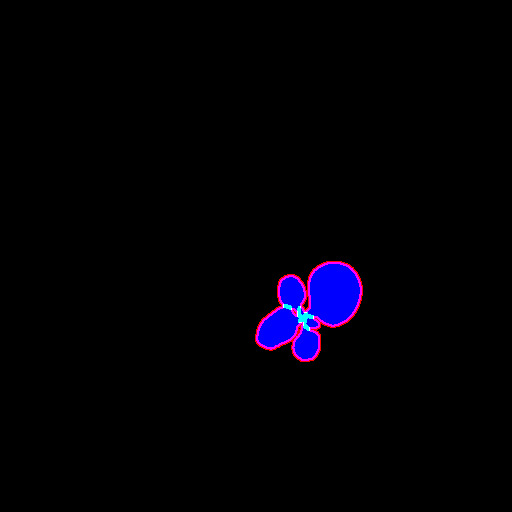
\includegraphics[width=\linewidth]{img/leaf/results-a3-7}} \\
        \UnframedBox{0.25\linewidth}{0.25\linewidth}{\includegraphics[width=\linewidth]{img/leaf/empty}}
        \FramedBox{0.25\linewidth}{0.25\linewidth}{\includegraphics[width=\linewidth]{img/leaf/results-a3-2}}
        \FramedBox{0.25\linewidth}{0.25\linewidth}{\includegraphics[width=\linewidth]{img/leaf/results-a3-8}} \\
        \caption{Visual example of LSC results for A3}
        \label{fig:07-cvppp-a3}
    \end{figure}
    \vfill
    \begin{figure}[H]
        \centering
        \FramedBox{.5cm}{0.25\linewidth}{Input}
        \FramedBox{.5cm}{0.25\linewidth}{CNN output}
        \FramedBox{.5cm}{0.25\linewidth}{Ground truth} \\
        \FramedBox{0.25\linewidth}{0.25\linewidth}{\includegraphics[width=\linewidth]{img/leaf/results-a4-0}}
        \FramedBox{0.25\linewidth}{0.25\linewidth}{\includegraphics[width=\linewidth]{img/leaf/results-a4-1}}
        \FramedBox{0.25\linewidth}{0.25\linewidth}{\includegraphics[width=\linewidth]{img/leaf/results-a4-7}} \\
        \UnframedBox{0.25\linewidth}{0.25\linewidth}{\includegraphics[width=\linewidth]{img/leaf/empty}}
        \FramedBox{0.25\linewidth}{0.25\linewidth}{\includegraphics[width=\linewidth]{img/leaf/results-a4-2}}
        \FramedBox{0.25\linewidth}{0.25\linewidth}{\includegraphics[width=\linewidth]{img/leaf/results-a4-8}} \\
        \caption{Visual example of LSC results for A4}
        \label{fig:07-cvppp-a4}
    \end{figure}
    \vfill
    
    \newpage
    The following table \ref{tab:lsc-detectron} reports method's results of different previous studies, to benchmark our method's results on this LSC dataset.
    
    \begin{table}[H]
        \centering
        \rowcolors{0}{gray!10}{white}
        \begin{tabularx}{\linewidth}{|X|r|c|}
            \hline
            \textbf{Study}                              & \textbf{SBD}    & \textbf{AbsDiffFG} \\ \hline
            \cite{ward2020scalable}     ward 2020       & \textbf{0.8800} &   -  \\
            \cite{kulikov2018instance}  kulikov 2018    & 0.8040 & 2.00 \\
            \cite{gomes2020leaf}        gomes 2020      & 0.7700 & \textbf{0.88} \\
            Ours method's results (2021)                & 0.7608 & 6.12 \\
            \cite{978-3-319-16220-1_5}  pape 2015       & 0.7440 & 2.60 \\
            \cite{scharr2016leaf}       scharr 2016     & 0.6830 & 3.80 \\
            \hline
        \end{tabularx}
        \caption{Comparison of our solution with state-of-the-art challengers in this dataset.}
        \label{tab:lsc-detectron}
    \end{table}
    
    These results show that the studied method is less efficient than \cite{ward2020scalable, kulikov2018instance} and \cite{gomes2020leaf}. Due to the small size of the training sample (102, 25, 22, 499 images for data subsets A1, A2, A3, A4, respectively), it can be assumed that this is due to the increase in data they use in order to expand their data set. It seems the data augmentation based on Perlin noise is insufficient. Nevertheless, our method is better than the following two: \cite{978-3-319-16220-1_5, scharr2016leaf}, since they don't use any data augmentation.
    However it can be noted that the $AbsDiffFG$ value for the studied method is much higher than for the others. This implies an important over-segmentation, resulting in particular from the quality of the A3 dataset as it can be seen in the table \ref{tab:eval-sub-cvppp}. 
    
    \subsection{Airphen dataset}
    
    The last one presented is our multispectral dataset, which contains variable acquisition conditions (sunny, cloudy, rainy, etc.), a variable number of leaves (from a few to hundreds), and contains very small leaves that touch or overlap the others. The next table \ref{tab:eval-Airphen} show the results of our method applied our dataset.
    
    \begin{table}[H]
        \rowcolors{0}{gray!10}{white}
        \begin{tabularx}{\linewidth}{|X|r|r|}
            \hline
            \textbf{Metric} 	& \textbf{Training} &  \textbf{Validation}  \\ \hline
            FgBgDice 	        &   0.9791 &   0.9785 \\
            BestDice 	        &   0.6744 &   0.6678 \\
            SBD 	            &   0.6670 &   0.6638 \\
            DiffFG 	        	& -41.3583 & -49.4667 \\
            AbsDiffFG       	&  46.7500 &  53.2333 \\ \hline
            Number of images 	&      240 &      60  \\
            Mean leaf count 	&   265.83 &  295.80  \\
            NAbsDiffFG          &   0.1758 &  0.1799  \\
            
            \hline
            % nombre de feuilles dans la vérité terrain
            %gt small leaf count 	&   38904 &  11633  \\
            %gt big leaf count 	    &   33927 &  5683  \\
            %gt small leaf mean 	&   162.1 &  190.7  \\
            %gt big leaf mean 	    &   141.4 &  93.16  \\
            %\hline
            % nombre de feuilles détectées
            %small leaf count 	&   24187 &  5073  \\
            %big leaf count 	    &   29761 &  83.16  \\
            %small leaf mean 	&   100.8 &  4647  \\
            %big leaf mean 	    &   124.0 &  76.18  \\
            %\hline
        \end{tabularx}
        \caption{Evaluation metrics for the Airphen dataset}
        \label{tab:eval-Airphen}
    \end{table}
    
    It can be seen that the $FGBGDice$ score shows adequate soil/vegetation segmentation, as demonstrated in our previous study \cite{Vayssade2021}. The scores $DiffFG$ and $AbsDiffFG$ show the presence of over-segmentation. This is due to two issues: the presence of small leaves and the advanced stage of mustard development. Indeed, the method sometimes confuses small leaves and large leaves, which implies in some cases under-segmentation for monocotyledons or over-segmentation for dycotyledons, probably generated by an imprecise annotation of classes. In the second case, this is due to the proposed loss function that forces over-segmentation, resulting in the detection of leaflets instead of leaves in the case of advanced mustard development, as showed in the figure \ref{fig:07-Airphen-0}. These errors imply that the $BestDice$ and $SBD$ scores are not as good as on the Komatsuna dataset and LSC Challenge, studied previously.
    
    \begin{figure}[H]
        \centering
        \FramedBox{.5cm}{0.25\linewidth}{Input}
        \FramedBox{.5cm}{0.25\linewidth}{CNN output}
        \FramedBox{.5cm}{0.25\linewidth}{Ground truth} \\
        
        \FramedBox{0.25\linewidth}{0.25\linewidth}{\includegraphics[width=\linewidth]{img/leaf/airphen-false}}
        \FramedBox{0.25\linewidth}{0.25\linewidth}{\includegraphics[width=\linewidth]{img/leaf/airphen-detection}}
        \FramedBox{0.25\linewidth}{0.25\linewidth}{\includegraphics[width=\linewidth]{img/leaf/airphen-gt-detection}} \\
        
        %%\FramedBox{0.25\linewidth}{.5cm}{\rotatebox[]{90}{body}}
        \UnframedBox{0.25\linewidth}{0.25\linewidth}{\includegraphics[width=\linewidth]{img/leaf/empty}}
        \FramedBox{0.25\linewidth}{0.25\linewidth}{\includegraphics[width=\linewidth]{img/leaf/airphen-body}}
        \FramedBox{0.25\linewidth}{0.25\linewidth}{\includegraphics[width=\linewidth]{img/leaf/airphen-gt-body}} \\
        
        %\FramedBox{0.25\linewidth}{0.25\linewidth}{\rotatebox[]{90}{Watershed}}
        %\FramedBox{0.25\linewidth}{0.25\linewidth}{\includegraphics[width=\linewidth]{img/leaf/airphen-watershed}}
        %\FramedBox{0.25\linewidth}{0.25\linewidth}{\includegraphics[width=\linewidth]{img/leaf/airphen-gt-watershed}} \\
        
        \caption{Example of the visual results for the Airphen dataset}
        \label{fig:07-Airphen-0}
    \end{figure}
    
    To show the difference and complexity of this dataset, the method developed by \cite{ward2020scalable} was also learned. This method is based on the Mask-RCNN. However, the method uses data augmentation based on a library that only supports 8-bit unsigned integers. Thus, data augmentation was disabled because the dataset uses a 32-bit float format. The following table \ref{tab:eval-Airphen-rcnn} shows these results.
    
    \begin{table}[H]
        \rowcolors{0}{gray!10}{white}
        \begin{tabularx}{\linewidth}{|X|r|r|}
            \hline
            \textbf{Metric} 	& \textbf{Training} &  \textbf{Validation}  \\ \hline
            FgBgDice 	        &    0.6266 &    0.6111 \\
            BestDice 	        &    0.2271 &    0.2157 \\
            SBD 	            &    0.2266 &    0.2149 \\
            DiffFG 	        	& -186.0292 & -217.0667 \\
            AbsDiffFG       	&  186.5542 &  217.1333 \\ \hline
            NAbsDiffFG       	&    0.7018 &    0.7341 \\ \hline
        \end{tabularx}
        \caption{Evaluation metrics for the Airphen dataset using Mask-RCNN}
        \label{tab:eval-Airphen-rcnn}
    \end{table}
    
    These results show that the method proposed by \cite{ward2020scalable} does not correctly detect leaves in a dense foliage environment. The $FgBgDice$ score shows that the soil/vegetation discrimination is weak. As well as the $BestDice$ and $SBD$ scores which shows poor detection of individuals segmentation mask. The $DiffFG$ and $AbsDiffFG$ scores confirm these results and show a large amount of undetected elements. As announced in the introduction, the methods based on object detection uses bounding box regressions and non-max suppression which strongly limit the detection in dense environment. Moreover the part of the network allowing to obtain the segmentation mask uses a fixed low resolution resulting in coarse segmentation masks. As shows in the figure \ref{fig:07-output}.
    
    \begin{figure}[H]
        \centering
        \FramedBox{.5cm}{0.22\linewidth}{Input}
        \FramedBox{.5cm}{0.22\linewidth}{Ground truth} 
        \FramedBox{.5cm}{0.22\linewidth}{CNN+Watershed}
        \FramedBox{.5cm}{0.22\linewidth}{Mask-RCNN} \\
        
        \FramedBox{0.22\linewidth}{0.22\linewidth}{\includegraphics[width=\linewidth]{img/leaf/airphen-false}}
        \FramedBox{0.22\linewidth}{0.22\linewidth}{\includegraphics[width=\linewidth]{img/leaf/airphen-gt-watershed}}
        \FramedBox{0.22\linewidth}{0.22\linewidth}{\includegraphics[width=\linewidth]{img/leaf/airphen-watershed}}
        \FramedBox{0.22\linewidth}{0.22\linewidth}{\includegraphics[width=\linewidth]{img/leaf/airphen-mrcnn}}
        
        
        \caption{Example of the Watershed output versus Mask-RCNN for Airphen dataset}
        \label{fig:07-output}
    \end{figure}
    
    \section{Discussion}
    \label{sec:07-discussion}
    
    In this study, we used different datasets. The Komatsuna dataset is composed only of mustard leaves at different stages of development acquired indoors under controlled acquisition conditions with a single camera. There are between 3 and 6 leaves per image for an average of $4.9$ leaves. The LSC dataset is decomposed into three sub-datasets of Arabidopsis-Thaliana and one of Rosette plants all at different stages of development. They are acquired indoors under controlled acquisition conditions with their own camera. There are between 2 and 16 leaves per image for an average of $13.5$ leaves. Our dataset is composed of bean plants and weeds. Beans are at a single stage of development while weeds are at different stages of development. The acquisitions were made outdoors under uncontrolled conditions. There are between $4$ and $777$ leaves per image with an average of $271.83$ leaves. This dataset is now available online\footnote{\url{https://data.inrae.fr/dataset.xhtml?persistentId=doi:10.15454/JMKP9S}} and may help other studies working on leaves segmentation in natural and complex situations.
    
    We are interested in the metric $NAbsDiffFG$ to compare the performances of our method on the different datasets. We see that for our dataset it is $0.1758, 0.1799$ for the LSC dataset and $0.1050$ for the Komatsuna dataset. We thus obtain good results for the Komatsuna dataset which is the simplest, we obtain an average result for our dataset which is the most complex and finally weaker results on the LSC dataset. This allows us to deduce that the lighting conditions as well as the number of leaves do not influence the performances. On the other hand, the use of several cameras, as on the LSC dataset, could be at the origin of the decrease in performance due to a variation in spatial resolution from one camera to another. We deduce that our method, designed to be used on complex data such as our dataset, gives results comparable to classical methods on other types of datasets.
    
    The CNN used in our method deliberately gives a coarse segmentation in order to maximize the detection and separation of large leaves. The smaller ones are therefore poorly detected (over-segmentation or undetected). These results are reflected in the fact that there is little over-segmentation and under-segmentation of large leaves due to the loss function introduced which takes into account the number of elements detected and their surface. However two problems are raised with the use of this loss function. First of all, it is subject to error jumps in order to avoid merging objects, which makes its optimization difficult and thus requires several learning sessions for an optimal result.
    
    \newpage
    On the other hand, avoiding merging causes over-segmentation in some cases, such as the mustard in our dataset that detects leaflets. At this time we cannot say whether this is problematic. It is possible that the leaflet scale is more relevant in terms of segmentation than the leaf for advanced stages of plant development.
    
    With the watershed used next, we improve the coarse detection provided by the CNN by extending the detected areas to the ideal soil/vegetation segmentation mask defined by the method developed in a previous study \cite{Vayssade2021}. This step allows the identification of the smallest leaves. Although the smallest elements, with a diameter of $0-2$ pixels, are still difficult to detect due to spectral mixing \cite{Louargant2017}. This is an important result as it allows to configure an acquisition system for a specific minimum size of leaves to detect. In this work, the remaining small leaves are already segmented as vegetation and can be considered as stable due to their sizes. Some features are still relevant to be extracted (such as the size of the leaf and its distance from the crop row) and should help in discriminating crop from weeds, other may suffer from the spectral mixing and become irrelevant (spectral signature, texture...).
    
    There is still an important type of error. Indeed, a single pixel can be at the origin of errors leading to a bad fusion between two areas. It would therefore be interesting to study structural analysis methods in order to overcome these deficiencies. A possible method would be to vectorize the contours and look for an algorithm to reconnect or split the contours for instance according to convexity singularities.
    
    The main interest of the proposed method is its efficiency on mixes of plant species, acquired with natural light. It will be integrated in a processing chain dedicated to the discrimination of crops and weeds in agronomic scenes. Indeed, the detected leaves can be classified according to a large set of criteria (spectral signature, morphological characteristics, texture, distance from the crop row). The underlying hypothesis is that these criteria are more stable at the scale of the leaf than at the scale of the plant. However, this approach has certain limitations when leaves overlap others, as the detected shapes would be heterogeneous. Multifoliate leaves could also be difficult to characterize. In that case, detecting leaflets instead of leaves may be more relevant. 
    
    \section{Conclusion}
    
    The presented work shows that the CNN network enhances the quality of the segmentation based on multispectral images. Indeed, the background is well removed due to the upstream network with IBF and UFA modules with an accuracy of $95-98\%$ of mIoU. Our method is effective in the majority of cases, such as the segmentation of unifoliate leaves like Arabidopsis-Thaliana and early developmental stages of plants. However, our method is not effective in the advanced stages of plant development, especially on mustard which has highly segmented leaves. In this case our method detects leaflets instead of leaves. Their identification is nevertheless relevant for the phenotyping or classification of weeds.
    
    We have seen that the developed method presents better SBD performances $+[1.66-7.89]\%$ compared to studies that do not use data augmentation. However, on small datasets, it presents lower SBD performances $-[4.32-11.92]\%$ compared to recent studies that use it. To make the method more consistent we will therefore focus on data augmentation. To improve the detection of classes it would be interesting to improve the upstream modules with attention mechanisms. This method would allow to correct the illumination of the images. As well as the use of a \textit{MIRNET} \cite{Zamir2020MIRNet} would allow to eliminate the noise. Finally, to improve the downstream modules, the use of \textit{Selective Kernel Convolution} \cite{Zamir2020MIRNet} would allow a better fusion of the multi-scale information instead of \textit{Universal Function Approximator}. We will then try to minimize the under-segmentation detected in our method, by using the \textit{Deep Watershed Transform for Instance Segmentation} method \cite{8099788}.
    
    A small performance loss for the developed method is seen on our dataset compared to Komatsuna and LSC dataset. It would be interesting to evaluate the reason(s) leading to this loss as it may come from the uncontrolled acquisition conditions, the multispectral nature of the images, the size differences between leaves or the important number of leaves in each images.
    
    In all cases, this approach should lead to an enhancement of features extraction which may improve crop/weed classification. These increased performances would lead to a better tracking of the weed flora. These algorithms show promising and robust results in natural acquisition conditions. The segmentation results are obtained fast enough to be used in a real-time crop/weed discrimination setting and could be embedded on a Unmanned Ground Vehicle (UGV) for quick and localised intervention. Applied on images acquired from an Unmanned Aerial Vehicle (UAV) this could be used for tool assisted plot management to help farmer in their decision making.
    
    %%%%%%%%%%%%%%%%%%
    
    \section{Further research}
    
    We defined the CNN architecture from the state of the art, adding components in an increasing development cycle.  Thus, we have not established the contribution of each block on this paper. The first 3 modules (iit, ibf, ufa) and the last sprb modules have been widely developed in our previous study about vegetation segmentation, each module have showed a contribution. But further research is undergoing to show the impacts of different modules on the upstream and downstream of the network, and the proposed loss function, and loss weights. This task must be automated trough an hyper-parameter optimization process which we did'nt explored wet. And the watershed algorithm used to refine the output must be added to the neural network, and part of this optimization process. Finally more advanced data augmentation could be explored.
    
    
    \section*{Data availability} The Airphen dataset used in this study have been released and it's publicly available at \url{https://data.inrae.fr/dataset.xhtml?persistentId=doi:10.15454/JMKP9S}, using Creative Common CC0 1.0 Public Domain Dedication licence
    
    %The programming code is available from a public gitlab repository (\url{https://gitlab.com/phd-thesis-adventice/codes/phd-segmentation-optimizer})
    
    \section*{Funds \& Conflicts of Interest}This project has received funding from the European Union's Horizon 2020 research and innovation program [grant agreement ID: 727321] (project acronym: IWMPRAISE) and from the French National Research Agency Challenge RoSE [grant agreement ID: ANR-17-ROSE-0002] (project acronym: ROSEAU). The authors declare no conflict of interest.
	
	\newpage
	\section{Conclusion de chapitre}
	
	Les résultats de cette étude montrent que l'approche proposée pour la segmentation des feuilles est intéressante sur plusieurs jeux de données accessibles en ligne et sur nos données. Elle génère d'excellents résultats sur les données de Komatsuna. En revanche, la méthode n'est pas parmi les meilleures lorsqu'elle est appliquée au jeu de données du LSC (Leaf Segmentation Challenge), mais elle reste quand même compétitive. Pour nos données multispectrales, dans le cadre du challenge RoSE, les résultats montrent qu'une approche traditionnelle, telle que les mask R-CNN qui reposent sur une utilisation de l'algorithme NMS ne permettent pas de détecter efficacement les individus en environnement dense. Contrairement à la méthode qui a été développée dans cet article. Cependant, bien que ces résultats représentent une avancée dans le domaine du ``pixelwise instance segmentation'', des recherches complémentaires doivent être entreprises.
    
    Concernant l'échelle de segmentation (i.e. la feuille), ces résultats suggèrent qu'une entité légèrement plus fine serait préférable d'un point de vue segmentation. En effet la visualisation des résultats sur les données du challenge RoSE, montre que les feuilles unifoliées/unilobées sont bien détectées, ce qui n'est pas le cas des feuilles multifoliées ou multilobées. Ainsi, l'échelle foliole serait probablement plus opportune.
    
    Le présent chapitre \ref{chap:deep-leaf} et le chapitre précédent \ref{chap:vegetation-indices} constituent l'étape de segmentation de notre pipeline. Maintenant, que l'on est capable de détecter les individus, nous nous intéresserons à l'extraction de propriétés et la classification, comme nous pouvons l'observer sur la figure ci-dessous.
	
	\begin{figure}[H]
		\tikzset{
	ppblock/.style={
		rectangle,
		minimum size=6mm,
		very thick,
		draw=black!50,
		text centered,
		font=\ttfamily,
		minimum width=8em,
		minimum height=6mm,
		top color=white,
	},
	%
	figure/.style={
		rectangle,
		rectangle split,
		rectangle split parts=2,
		very thick,
		draw=black!50,
		text centered,
		append after command={
			\pgfextra
			\fill[top color=#1, bottom color=#1]
			(\tikzlastnode.one west) 
			[rounded corners] |- (\tikzlastnode.north) -| (\tikzlastnode.one east) 
			[sharp corners]   |- (\tikzlastnode.one split) -| cycle;
			\fill[top color=white, bottom color=#1]
			(\tikzlastnode.two west) 
			[rounded corners] |- (\tikzlastnode.south) -| (\tikzlastnode.two east)  
			[sharp corners]   |- (\tikzlastnode.one split) -| cycle;
			\endpgfextra
		},
	},
    splitted/.style={
        rectangle,
        rectangle split,
        rectangle split horizontal,
        rectangle split parts=2,
        very thick,
        draw=black!50,
        text centered,
        append after command={
            \pgfextra
            \fill[top color=white, bottom color=#1]
            (\tikzlastnode.south)
            [rounded corners] -| (\tikzlastnode.west) |- (\tikzlastnode.one north)
            [sharp corners]   -| (\tikzlastnode.one split) |- cycle;
            \fill[top color=white, bottom color=#1]
            (\tikzlastnode.two south)
            [rounded corners] -| (\tikzlastnode.east) |- (\tikzlastnode.north)
            [sharp corners]   -| (\tikzlastnode.one split) |- cycle;
            \endpgfextra
        },
    },
	%
	static/.style={ppblock, bottom color={black!20}},
	nonterminal/.style={ppblock, bottom color={blue!30}},
	terminal/.style={ppblock, bottom color={green!20}},
	algorithm/.style={ppblock, bottom color={yellow!50}},
	error/.style={ppblock, bottom color={red!20}},
	type/.style={ppblock, bottom color={red!20}},
	loss/.style={ppblock, dashed, bottom color={black!20}, font=\itshape},
	%
	tiny/.style={
		rounded rectangle,
		very thick,
		draw=black!50,
		top color=white,
		bottom color=red!20,
        text centered,
		font=\ttfamily,
	},
    operator/.style = {
        circle,
        scale=0.6,
        draw=black!50,
        top color=white,
        bottom color=red!20,
        font=\boldmath,
    },
	%
	skip loop/.style={to path={-- ++(0,#1) -| (\tikztotarget)}}
}
		\centering
		\begin{tikzpicture}[
		>=stealth',thick,
		tip/.style={->,shorten >=0.007pt},
		every node/.style={scale=0.8},
		]
		\matrix (table) [matrix of nodes, column sep=6mm, row sep=2mm, align=center] {
            \node (p07) [terminal]   {{\faShare*} Pre-Processing};      &
            \node (p08) [terminal]   {{\faPagelines} Deep Indices};       &
            \node (p09) [terminal]   {{\faLeaf} Deep Leaves};        &
            \node (p10) [algorithm]   {{\faCalculator} Features};           &
            \node (p11) [algorithm]   {{\faChartPie} Data Mining};        \\
		};
		
		\draw[->]     (p07) to (p08);
		\draw[->]     (p08) to (p09);
		\draw[->]     (p09) to (p10);
		\draw[->]     (p10) to (p11);
		\end{tikzpicture}
		
        {Rappel de l'architecture de notre chaîne fonctionnelle \\ ici les premières étapes en vert sont terminées, et en jaune les étapes suivantes étudiées}
	\end{figure}
	
\end{document}

